% Befehl \fibelvorstellung: Erstellt die Vorstellung eines FSlers mit Bild
%	Parameter #1: Bild (wrapfigure)
%	Parameter #2: Text
\newcommand{\fibelvorstellung}[2]{%
	\begin{minipage}{\columnwidth}
		% Kein Abstand vor bzw. nach Bildern bei wrapfigure
		\setlength{\intextsep}{0cm}
		% geringfügiger Abstand zwischen Paragraphen
		\setlength{\parskip}{0.5ex}
		#1
		#2
		\vspace{0.5ex}
	\end{minipage}
	
	\vspace{5ex plus 2ex minus 1ex}
}
\newlength{\fibelstdlen}
\setlength{\fibelstdlen}{3.7cm}

\section{Der Fachschaftsrat~(FSR) Physik stellt sich vor}
\begin{multicols*}{2}

\fibelvorstellung{
	\begin{wrapfigure}{l}{0cm}
		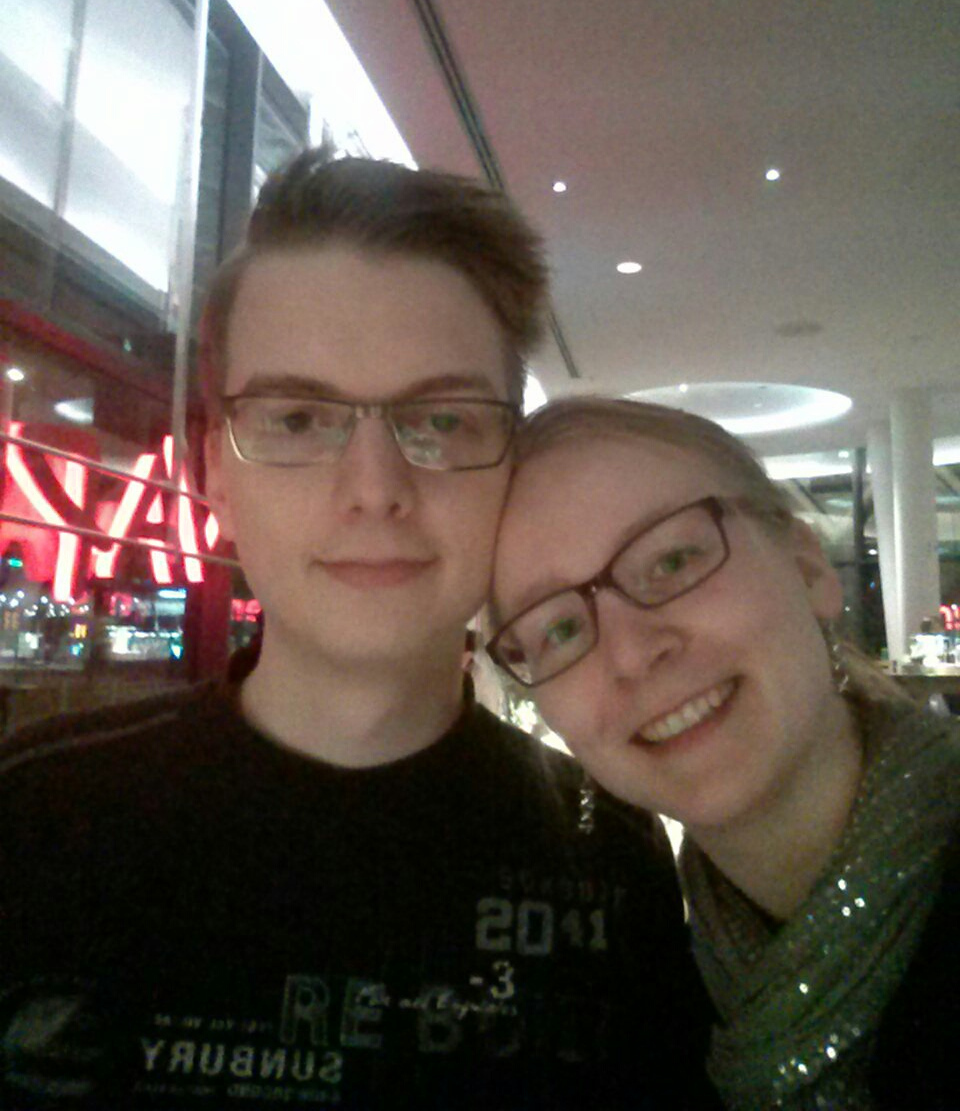
\includegraphics[width=5.1cm]{res/vorstellungsfotos/simon_may_alexandra_everwand_edited_cropped.jpg}
	\end{wrapfigure}
}
{% LaTeX-Warnung deaktivieren
%\hbadness=10000
Hey, wir sind Alex (rechts) und Simon (links), das "Fachschaftspärchen". Da man uns eigentlich nie getrennt antreffen kann, stellen wir uns hier gemeinsam vor -- das kommt der Realität näher ;-)

Wir starten beide in unser 9.~Semester an der Uni und sind vor Kurzem aus unserem Jahr in Schweden zurückgekommen. Ich (Simon) kann euch bei technischen und Computer-bezogenen Fragen weiterhelfen; ich (Alex) organisiere z.\,B.\ den Buchmarkt und die Spieleabende. Fragt aber auch sonst ruhig nach, wenn ihr Hilfe braucht :-)}
	
\fibelvorstellung{
	\begin{wrapfigure}{r}{0cm}
		\includegraphics[width=\fibelstdlen]{res/vorstellungsfotos/benedikt_bieringer.png}
	\end{wrapfigure}
}
{Hallo zusammen! Mein Name ist Benedikt. In der Fachschaft bin ich für so ziemlich alles verantwortlich, was mit Computergrafik/Design zu tun hat. Programmieren und Schwimmen sind nur zwei meiner weiteren Freizeitbeschäftigungen. In meinen jetzt 4~Semestern Fachschafts- und Studienerfahrung kann ich euch aber auch bei einer ganzen Reihe weiterer Fragen weiterhelfen.}

\fibelvorstellung{
	\begin{wrapfigure}{l}{0cm}
		\includegraphics[width=3.4cm]{res/vorstellungsfotos/bernd_hofschroeer.png}
	\end{wrapfigure}
}
{Ich bin Bernd, bin im 1.~Master-Semester und studiere Zweifachbachelor Physik--Chemie, werde also Lehrer.
Wenn ihr dazu Fragen habt, fragt!
Ansonsten bin ich seit meinem 3.~Semester in der Fachschaft!
\vspace{2\baselineskip}}

\fibelvorstellung{
	\begin{wrapfigure}{r}{0cm}
		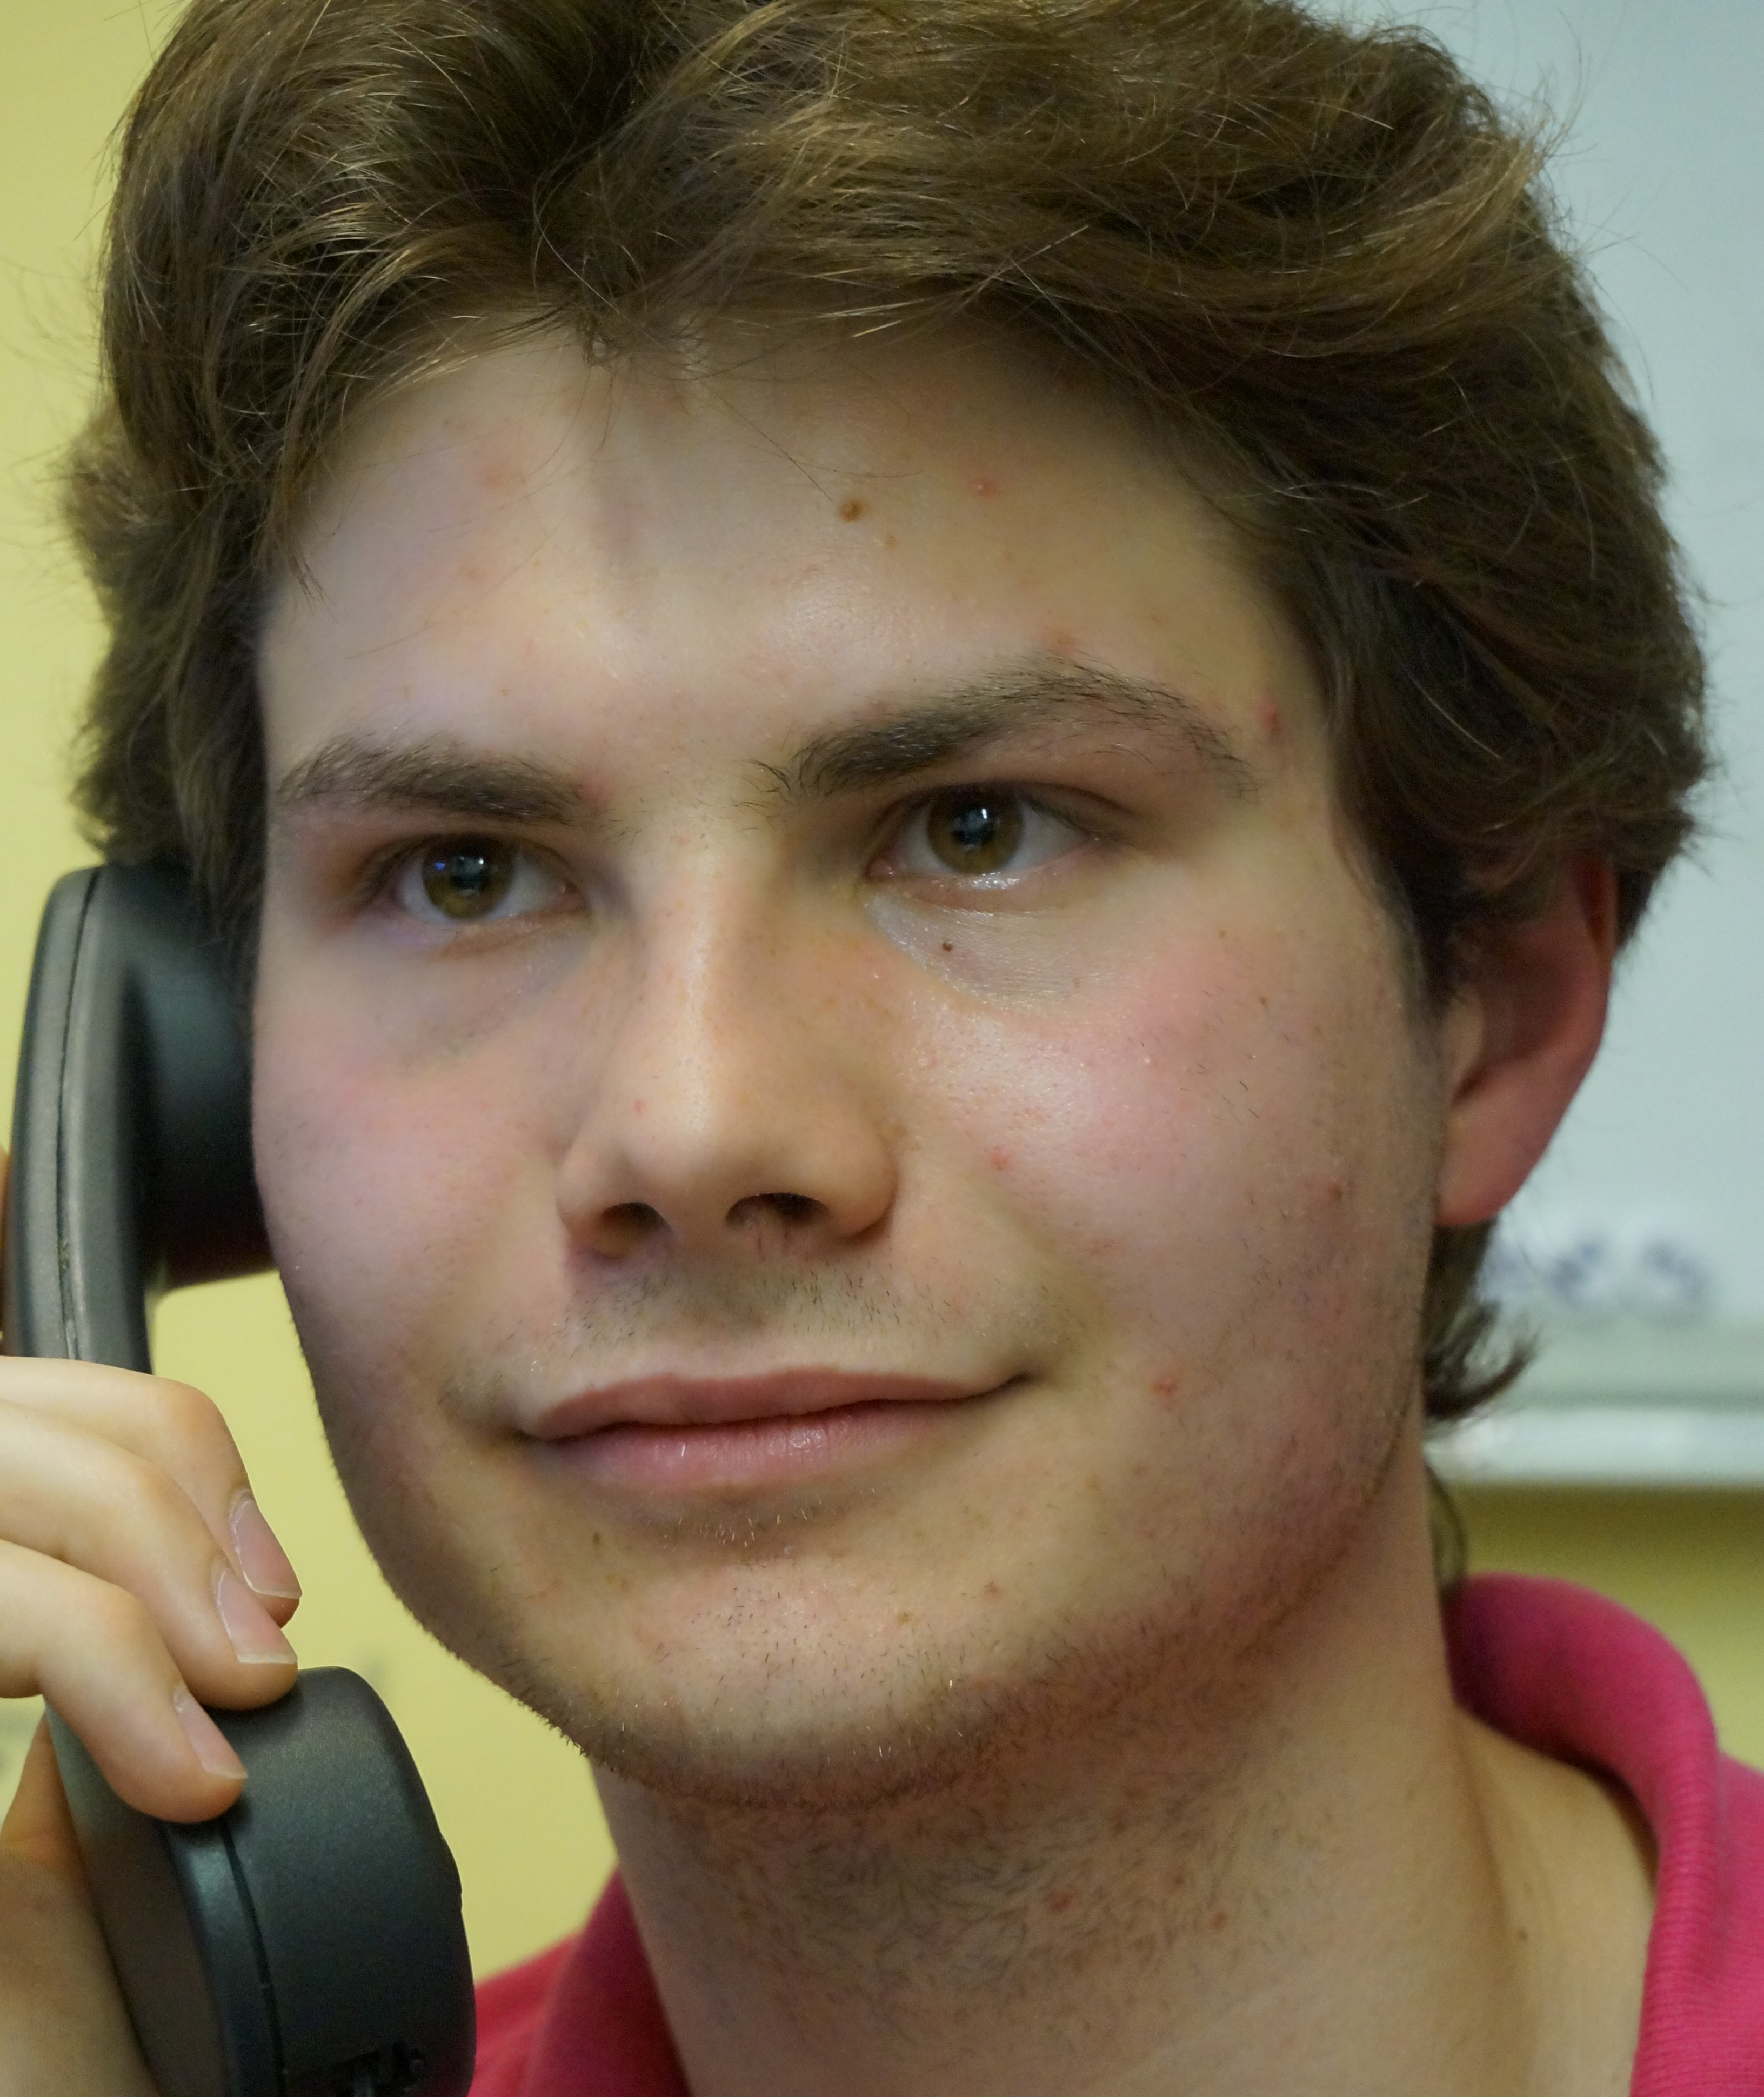
\includegraphics[width=3.5cm]{res/vorstellungsfotos/fabian_breitschwerdt_cropped.jpg}
	\end{wrapfigure}
}
{Hi Leute! Ich bin Fabian und für mich hat mittlerweile schon das 9.~Semester hier angebrochen; genauso lang bin ich auch in der Fachschaft. Mit Fragen könnt ihr immer gern zu mir kommen.
\vspace{2\baselineskip}}


\fibelvorstellung{
	\begin{wrapfigure}{l}{0cm}
		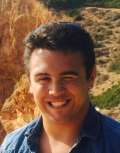
\includegraphics[width=\fibelstdlen]{res/vorstellungsfotos/fernando_romahn.png}
	\end{wrapfigure}
}
{Hallo liebe Erstis, ich bin (Europameister) Fernando, studiere seit vier Semestern Physik und bin ebenso lang in der Fachschaft.
Für gewöhnlich bin ich ein tiefenentspannter, gut gelaunter Fachschaftler, der von Stress und langfristiger Planung nicht viel hält.
Für Fragen, Probleme, Anregungen und Lobeshymnen auf mich stehe ich euch gern zur Verfügung :)}

\fibelvorstellung{
	\begin{wrapfigure}{r}{0cm}
		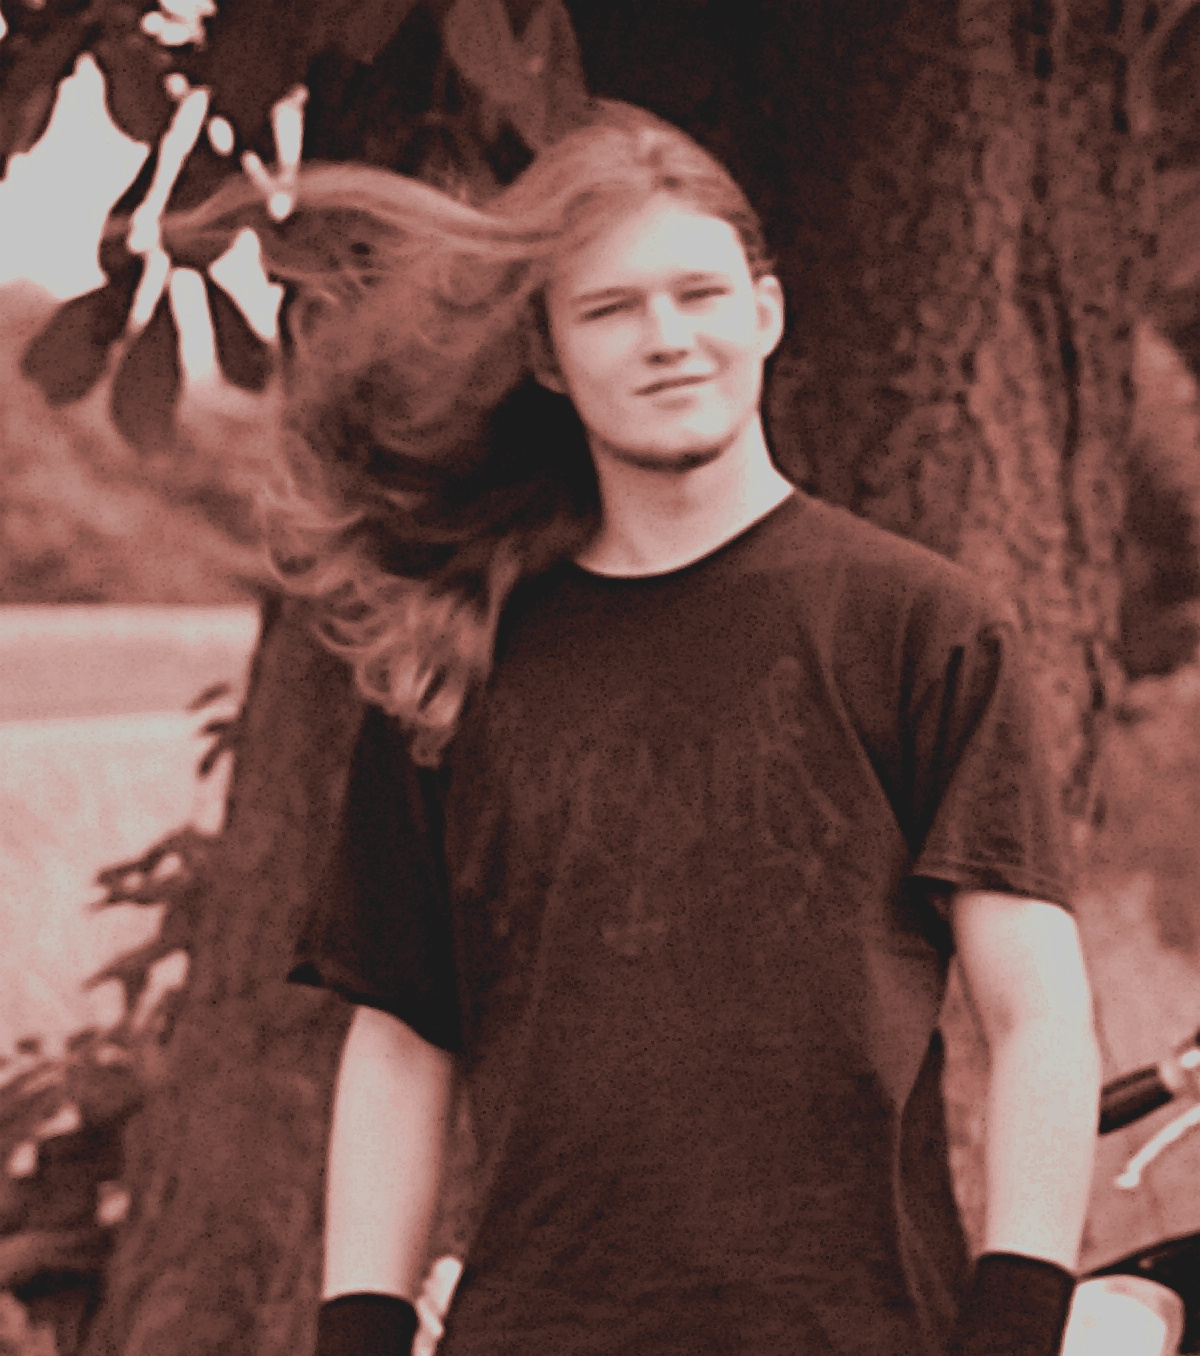
\includegraphics[width=\fibelstdlen]{res/vorstellungsfotos/jan_honermann_cropped.jpg}
	\end{wrapfigure}
}
{Hi, ich bin Jan und studiere jetzt Physik im 9.~Semester und bin seit drei Jahren in der Fachschaft tätig.
Falls ihr Fragen habt, könnt ihr euch gerne an mich wenden, ich bin auch meistens netter als ich aussehe ;)
\vspace{\baselineskip}}


\fibelvorstellung{
	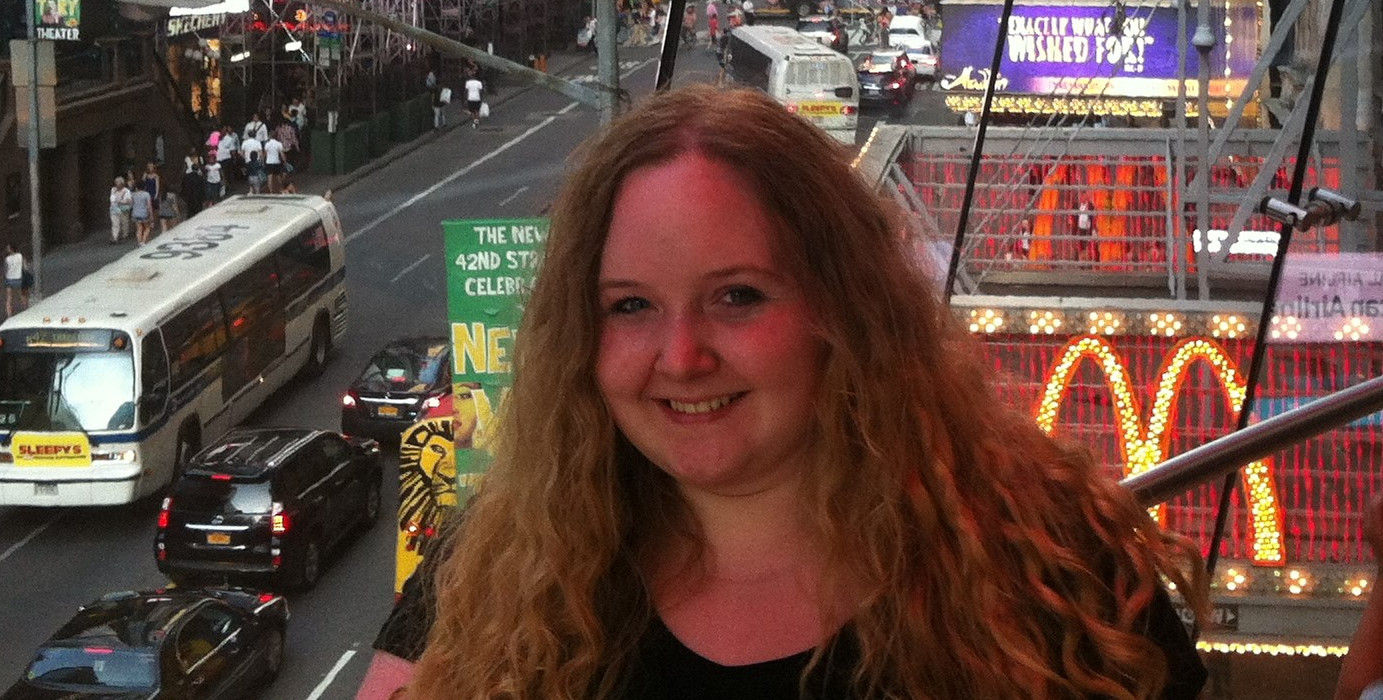
\includegraphics[width=\columnwidth]{res/vorstellungsfotos/jennifer_borcherding_cropped.jpg}
}
{Hey, ich bin Jenny und studiere jetzt im 3.~Semester Physik.
Ich bin seit einem Jahr in der Fachschaft und bei Fragen könnt ihr euch immer gerne an mich wenden.
Habt ganz viel Spaß in eurer Ersti-Woche und viel Erfolg im Studium!}

\fibelvorstellung{
	\begin{wrapfigure}{l}{0cm}
		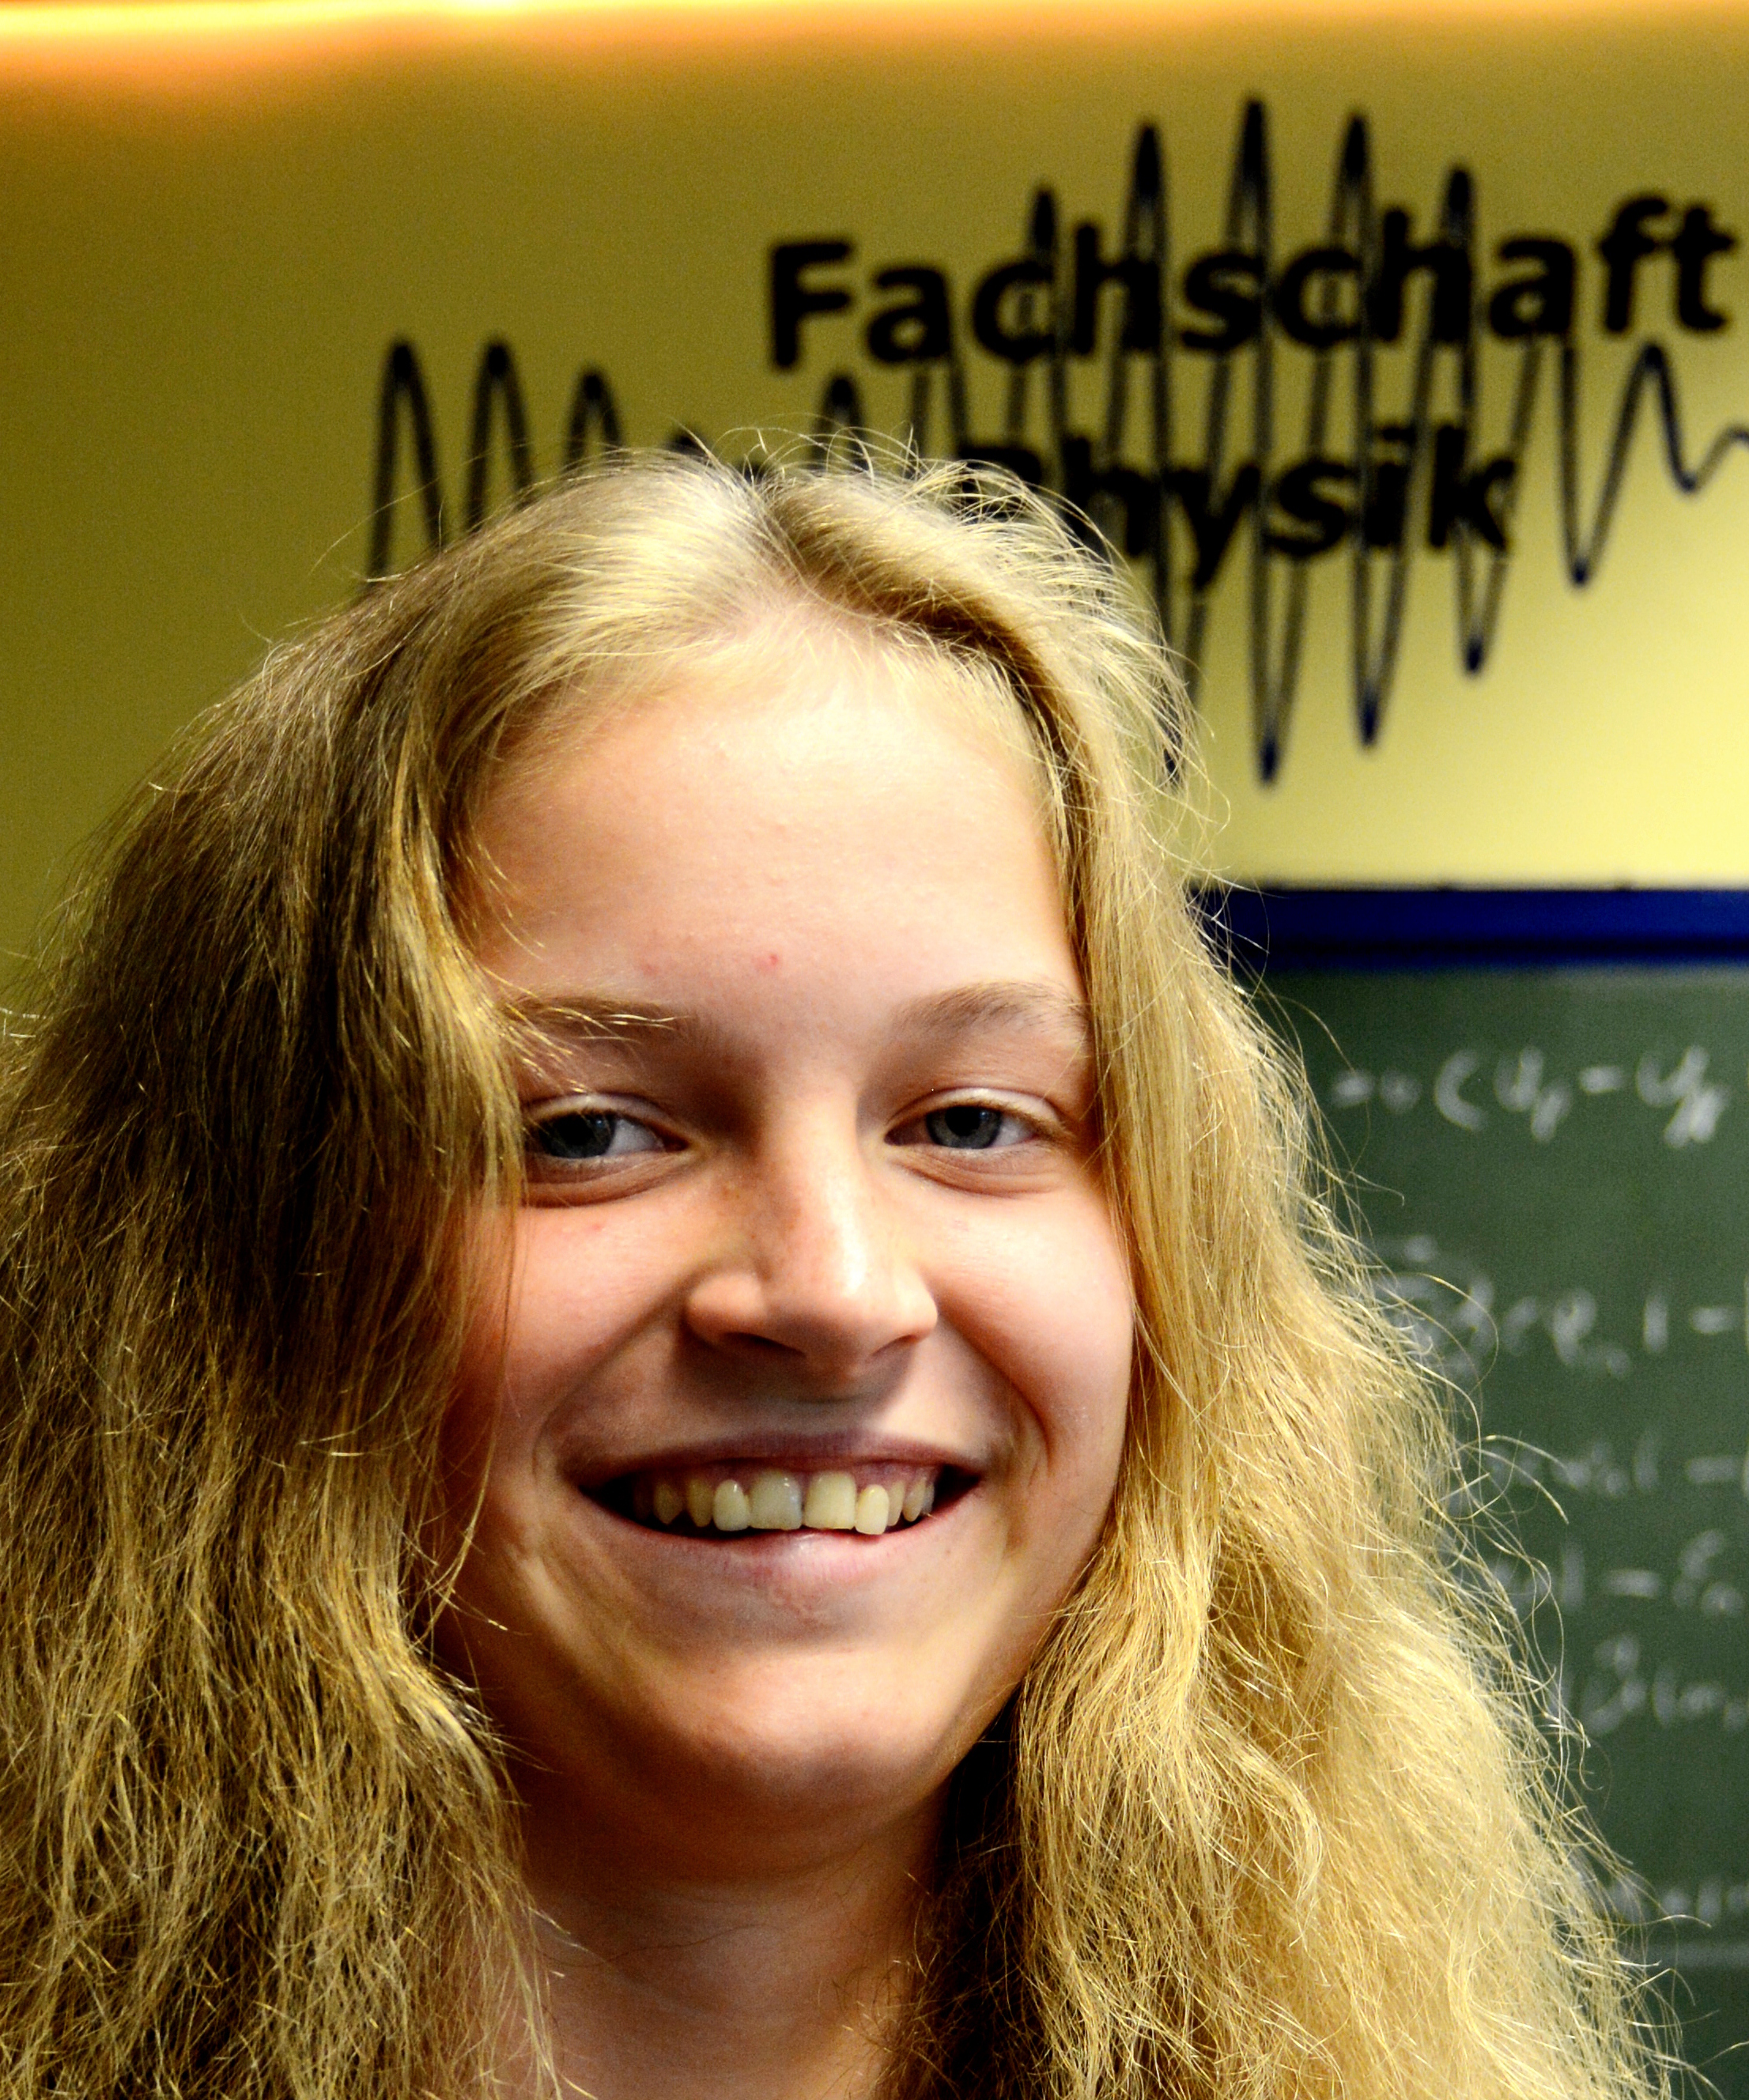
\includegraphics[width=\fibelstdlen]{res/vorstellungsfotos/johanna_jakob_cropped.jpg}
	\end{wrapfigure}
}
{Hi! Ich bin Johanna und starte jetzt mit dem dritten Semester vom 1Fach-Bachelor Physik.
In der Fachschaft bin ich quasi von Anfang an gerne mit dabei.
\vspace{3\baselineskip}}

\fibelvorstellung{
	\begin{wrapfigure}{r}{0cm}
		\includegraphics[width=\fibelstdlen]{res/vorstellungsfotos/lutz_althueser_cropped.jpg}
	\end{wrapfigure}
}
{Haii! Ich bin Lutz und mittlerweile am Ende des Masterstudiums angelangt.
Der Fachschaft bin ich vor unvorstellbaren 4~Jahren in meinem eigenen ersten Semester beigetreten.
In der Fachschaft werdet Ihr mich nur noch selten antreffen, dafür bin ich aber jederzeit in meinem Büro und kann bei jeder Angelegenheit helfen.
Neben vielen kleinen Aufgaben kümmere ich mich hauptsächlich um die Evaluation der Lehre und sorge somit dafür, dass die Vorlesungen so zufriedenstellend wie nur möglich gehalten werden!
Also bis bald!}

\fibelvorstellung{
	\begin{wrapfigure}{l}{0cm}
		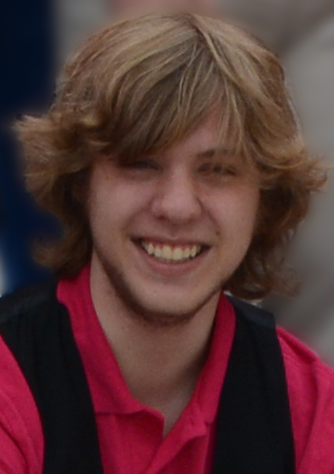
\includegraphics[width=\fibelstdlen]{res/vorstellungsfotos/jonas_kausch.png}
	\end{wrapfigure}
}
{Das ist Justus. Eigentlich heißt der Fachschafts-Doctor im 5.~Semester Jonas.
Prinzipiell ist er immer für eine ausgiebige Diskussion zu haben, sei es zu "Doctor Who", den Feinheiten der Kampfsysteme des antiken Griechenlands oder einem beliebigen anderen Thema, mit dem er sich selbstverständlich auskennt.
Allerdings ist er nicht immer besonders zuverlässig -- deswegen berichtet er hier nicht selbst über sich ;-)}

\begin{center}
	
\includegraphics[width=\columnwidth]{res/fsphys_logo.pdf}
\end{center}

\fibelvorstellung{
	\begin{wrapfigure}{r}{0cm}
		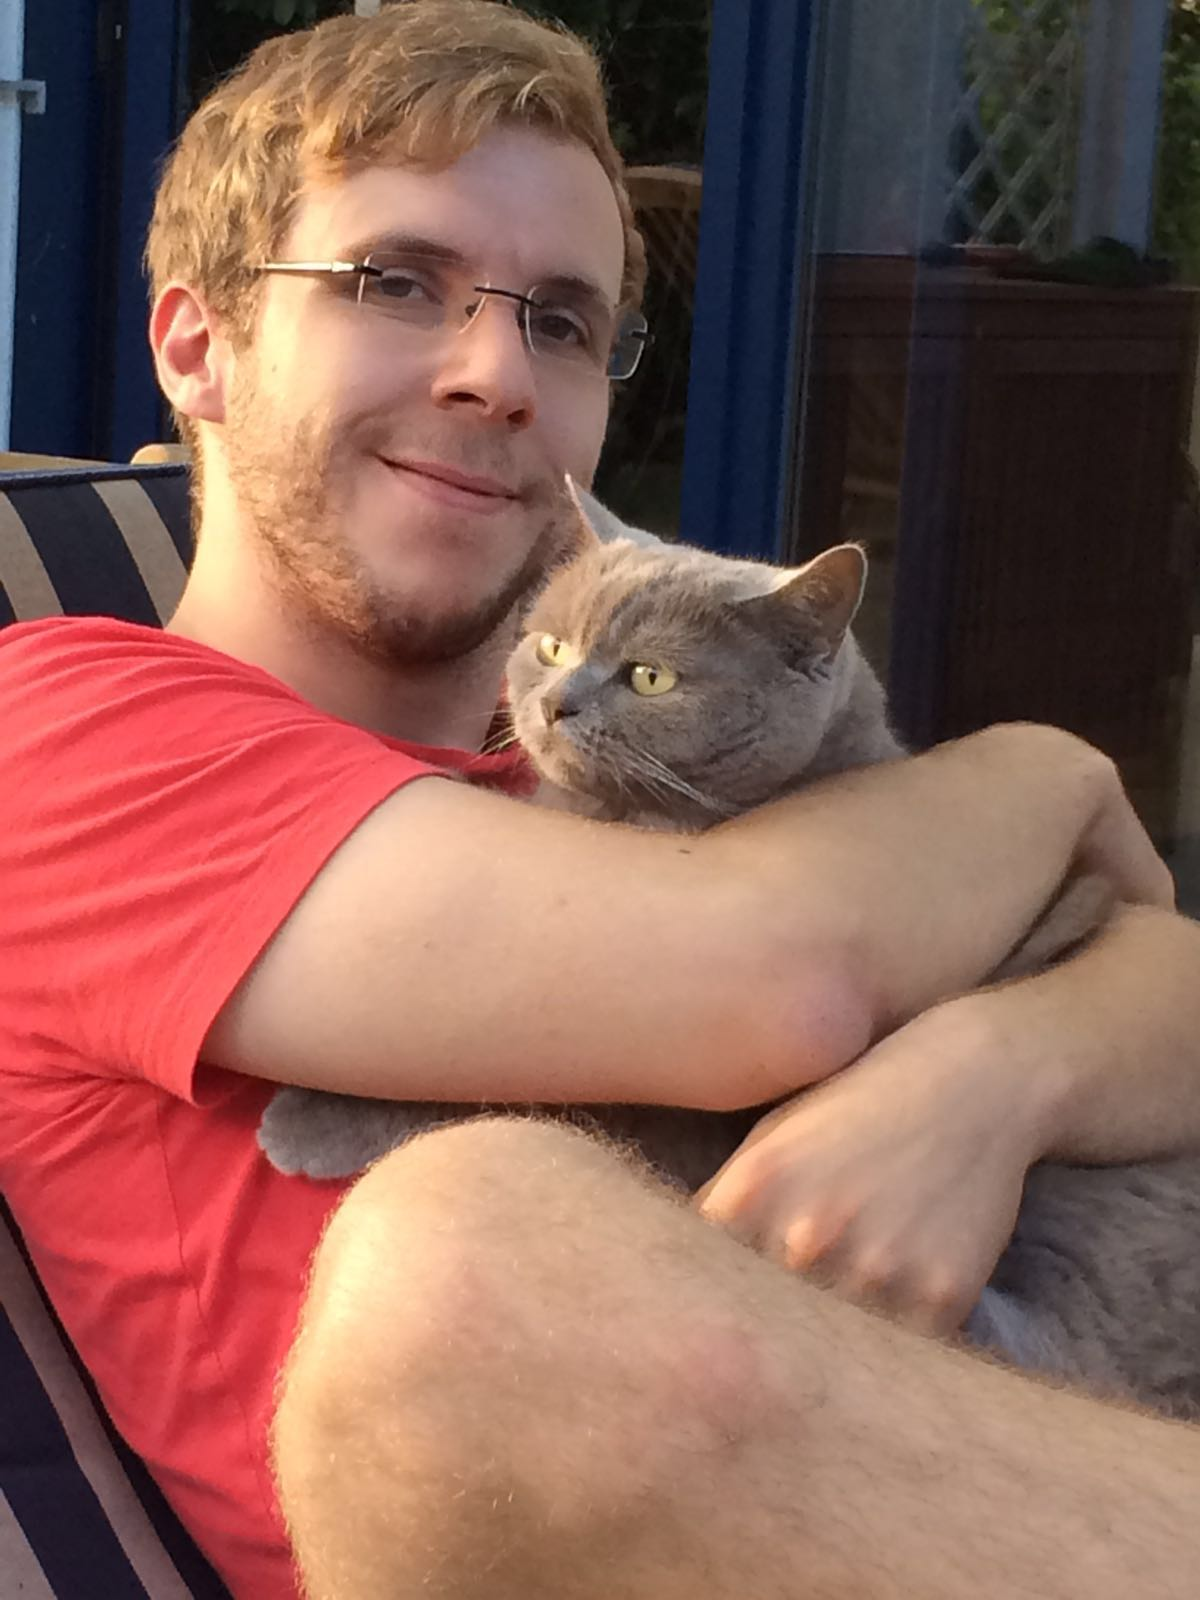
\includegraphics[width=\fibelstdlen]{res/vorstellungsfotos/lukas_eschmann.jpg}
	\end{wrapfigure}
}
{Hey hey, ich bin Lukas und im 9.~Semester und so lange auch in der Fachschaft aktiv.
Mittlerweile bekleide ich das Amt des Vorsitzenden, organisiere das Sommerfest und bin im Lehrpreiskomitee und hab viel Spaß dabei.
Privat geh ich viel tanzen (also nicht zappeln in der Disco) und sitz auch gerne noch lange nach Fachschaftssitzungen mit den anderen hier vorgestellten Fachschaftlern auf n Bierchen in der Fachschaft.
Wenn ihr Lust habt, schaut doch auch mal vorbei.
Wie immer freue ich mich auch dieses Jahr ganz besonders auf eure O-Woche, euer Ersti-Wochenende und natürlich auch auf euch.}

\fibelvorstellung{
	\begin{wrapfigure}{l}{0cm}
		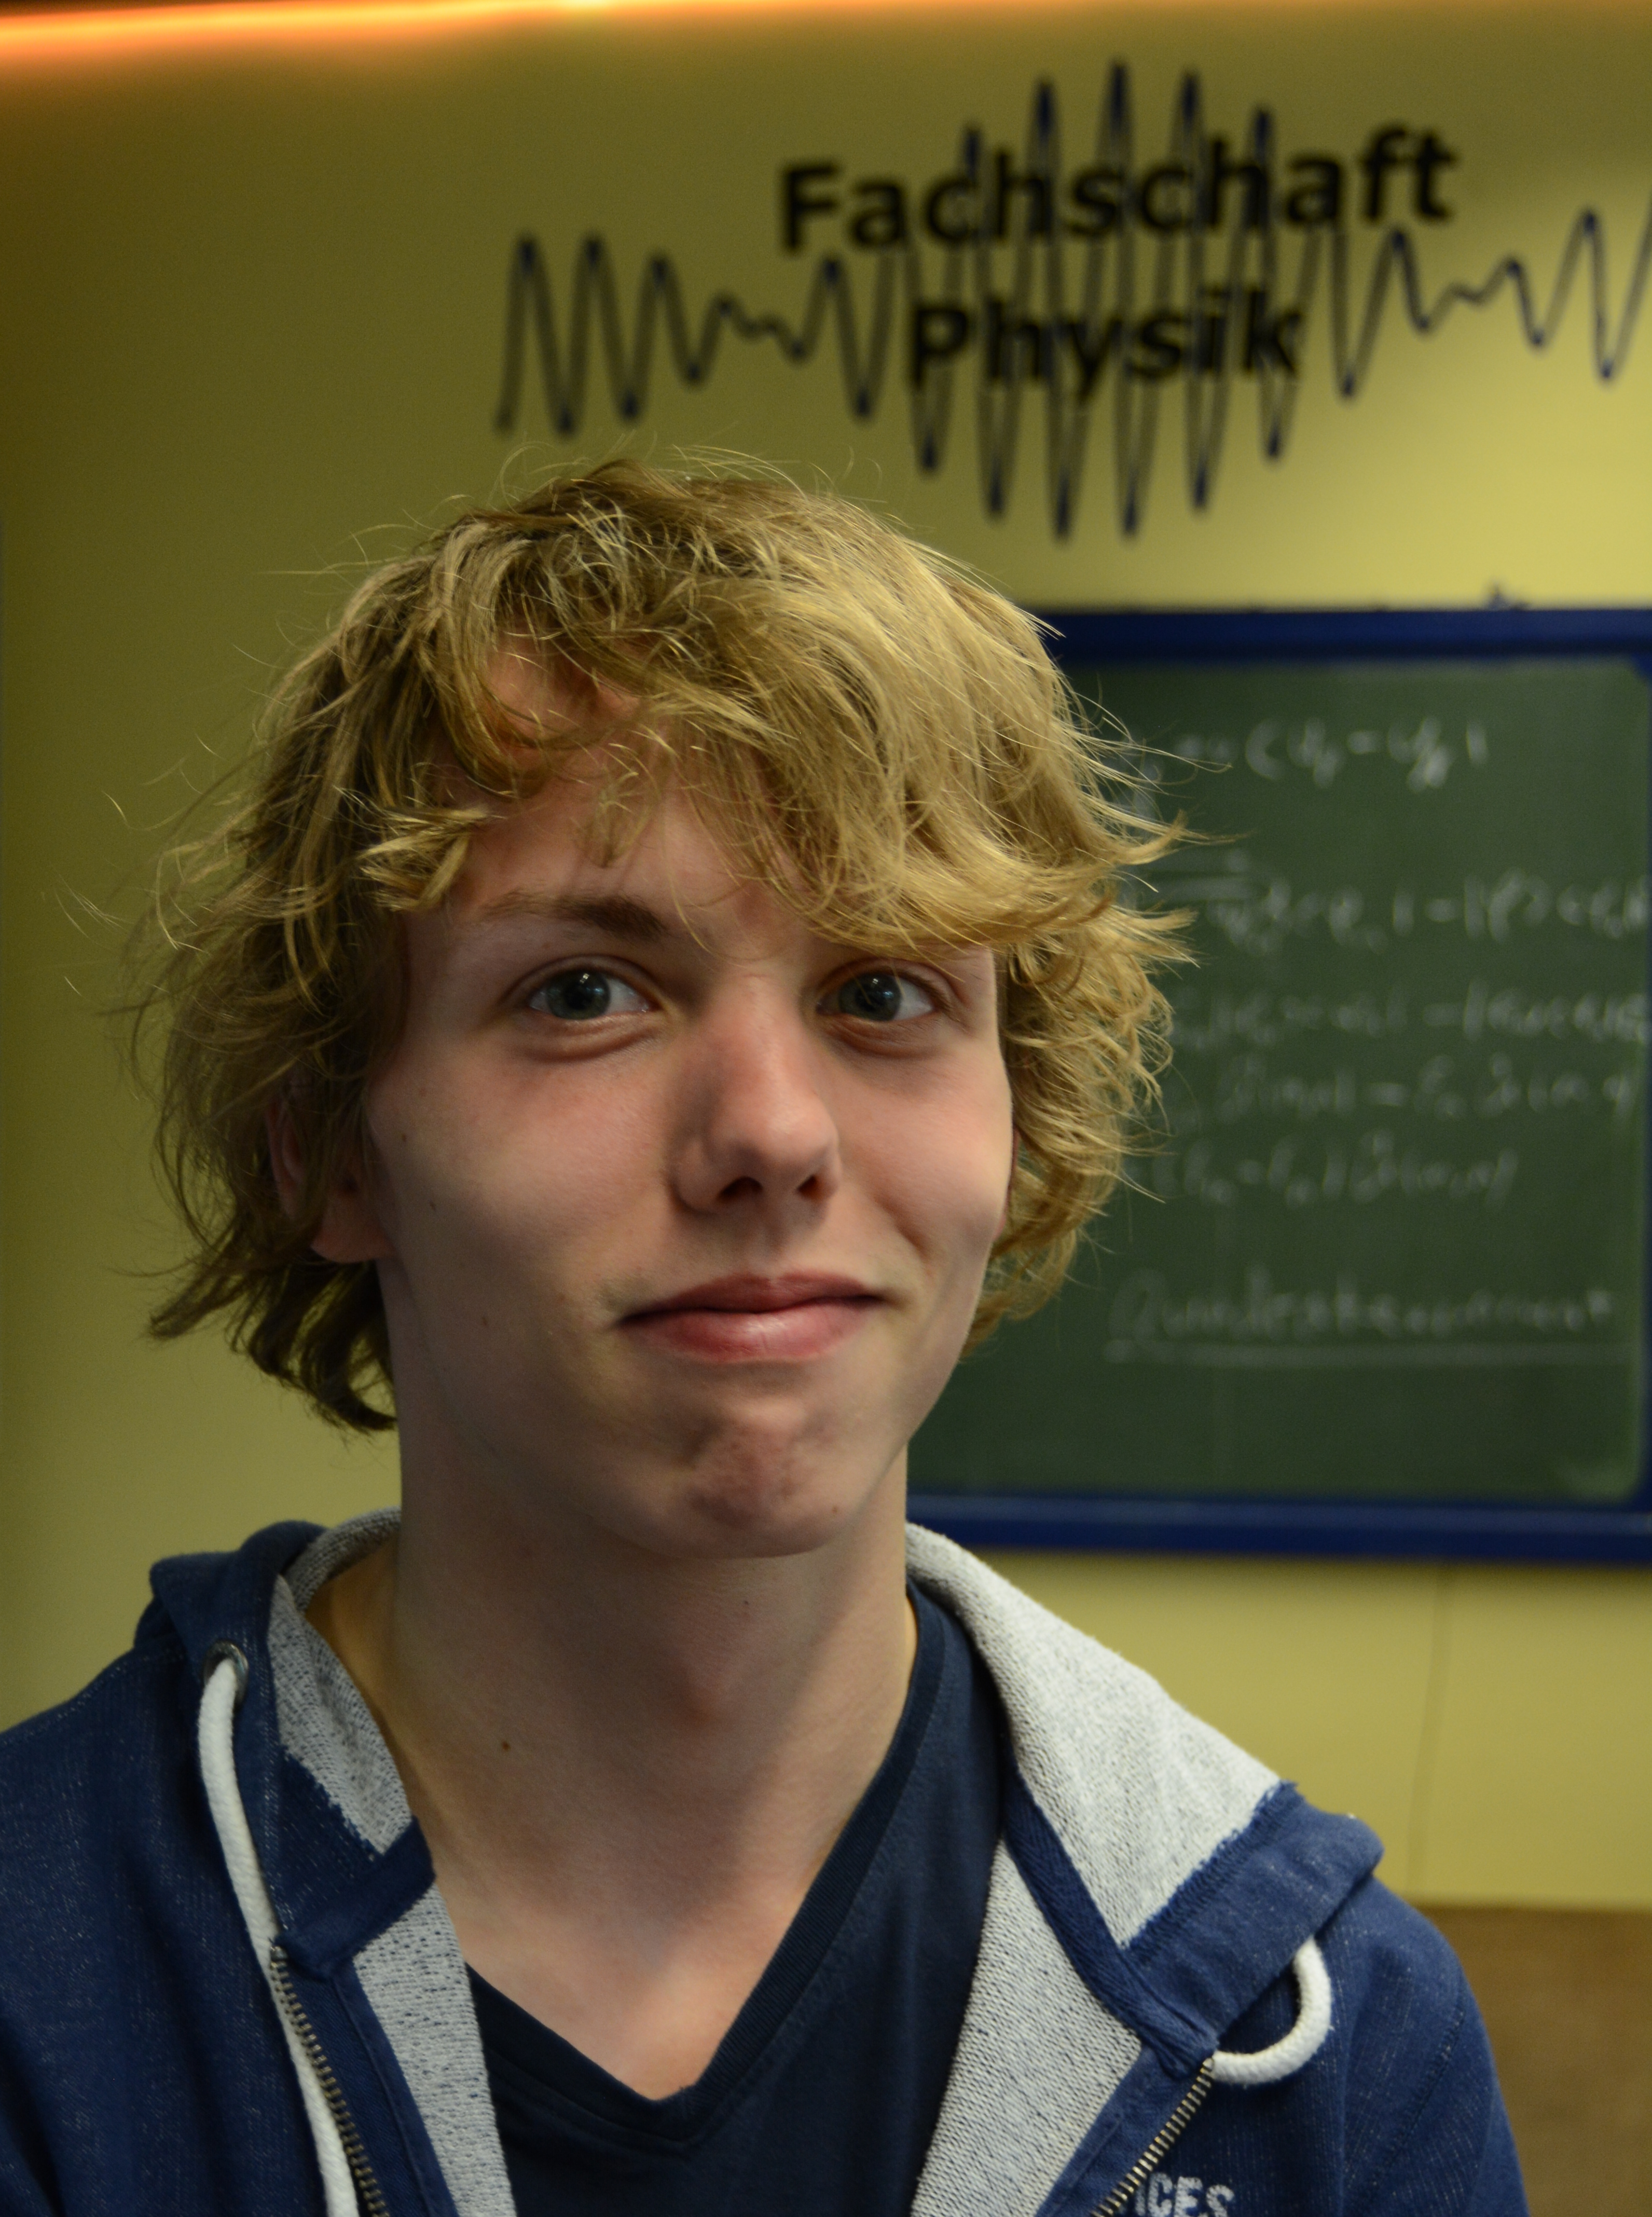
\includegraphics[width=\fibelstdlen]{res/vorstellungsfotos/marius_willer_cropped.jpg}
	\end{wrapfigure}
}
{Hi, ich bin Marius und heiße euch ebenfalls hier an der Uni Münster im Fachbereich Physik willkommen. 
Auch ich habe die Ersti-Woche sehr genossen und die Ersti--Fahrt/das Ersti-Wochenende war auch unbeschreiblich cool.
Ich hoffe, ihr werdet euren "Spaß" hier haben.}

\fibelvorstellung{
	\begin{wrapfigure}{r}{0cm}
		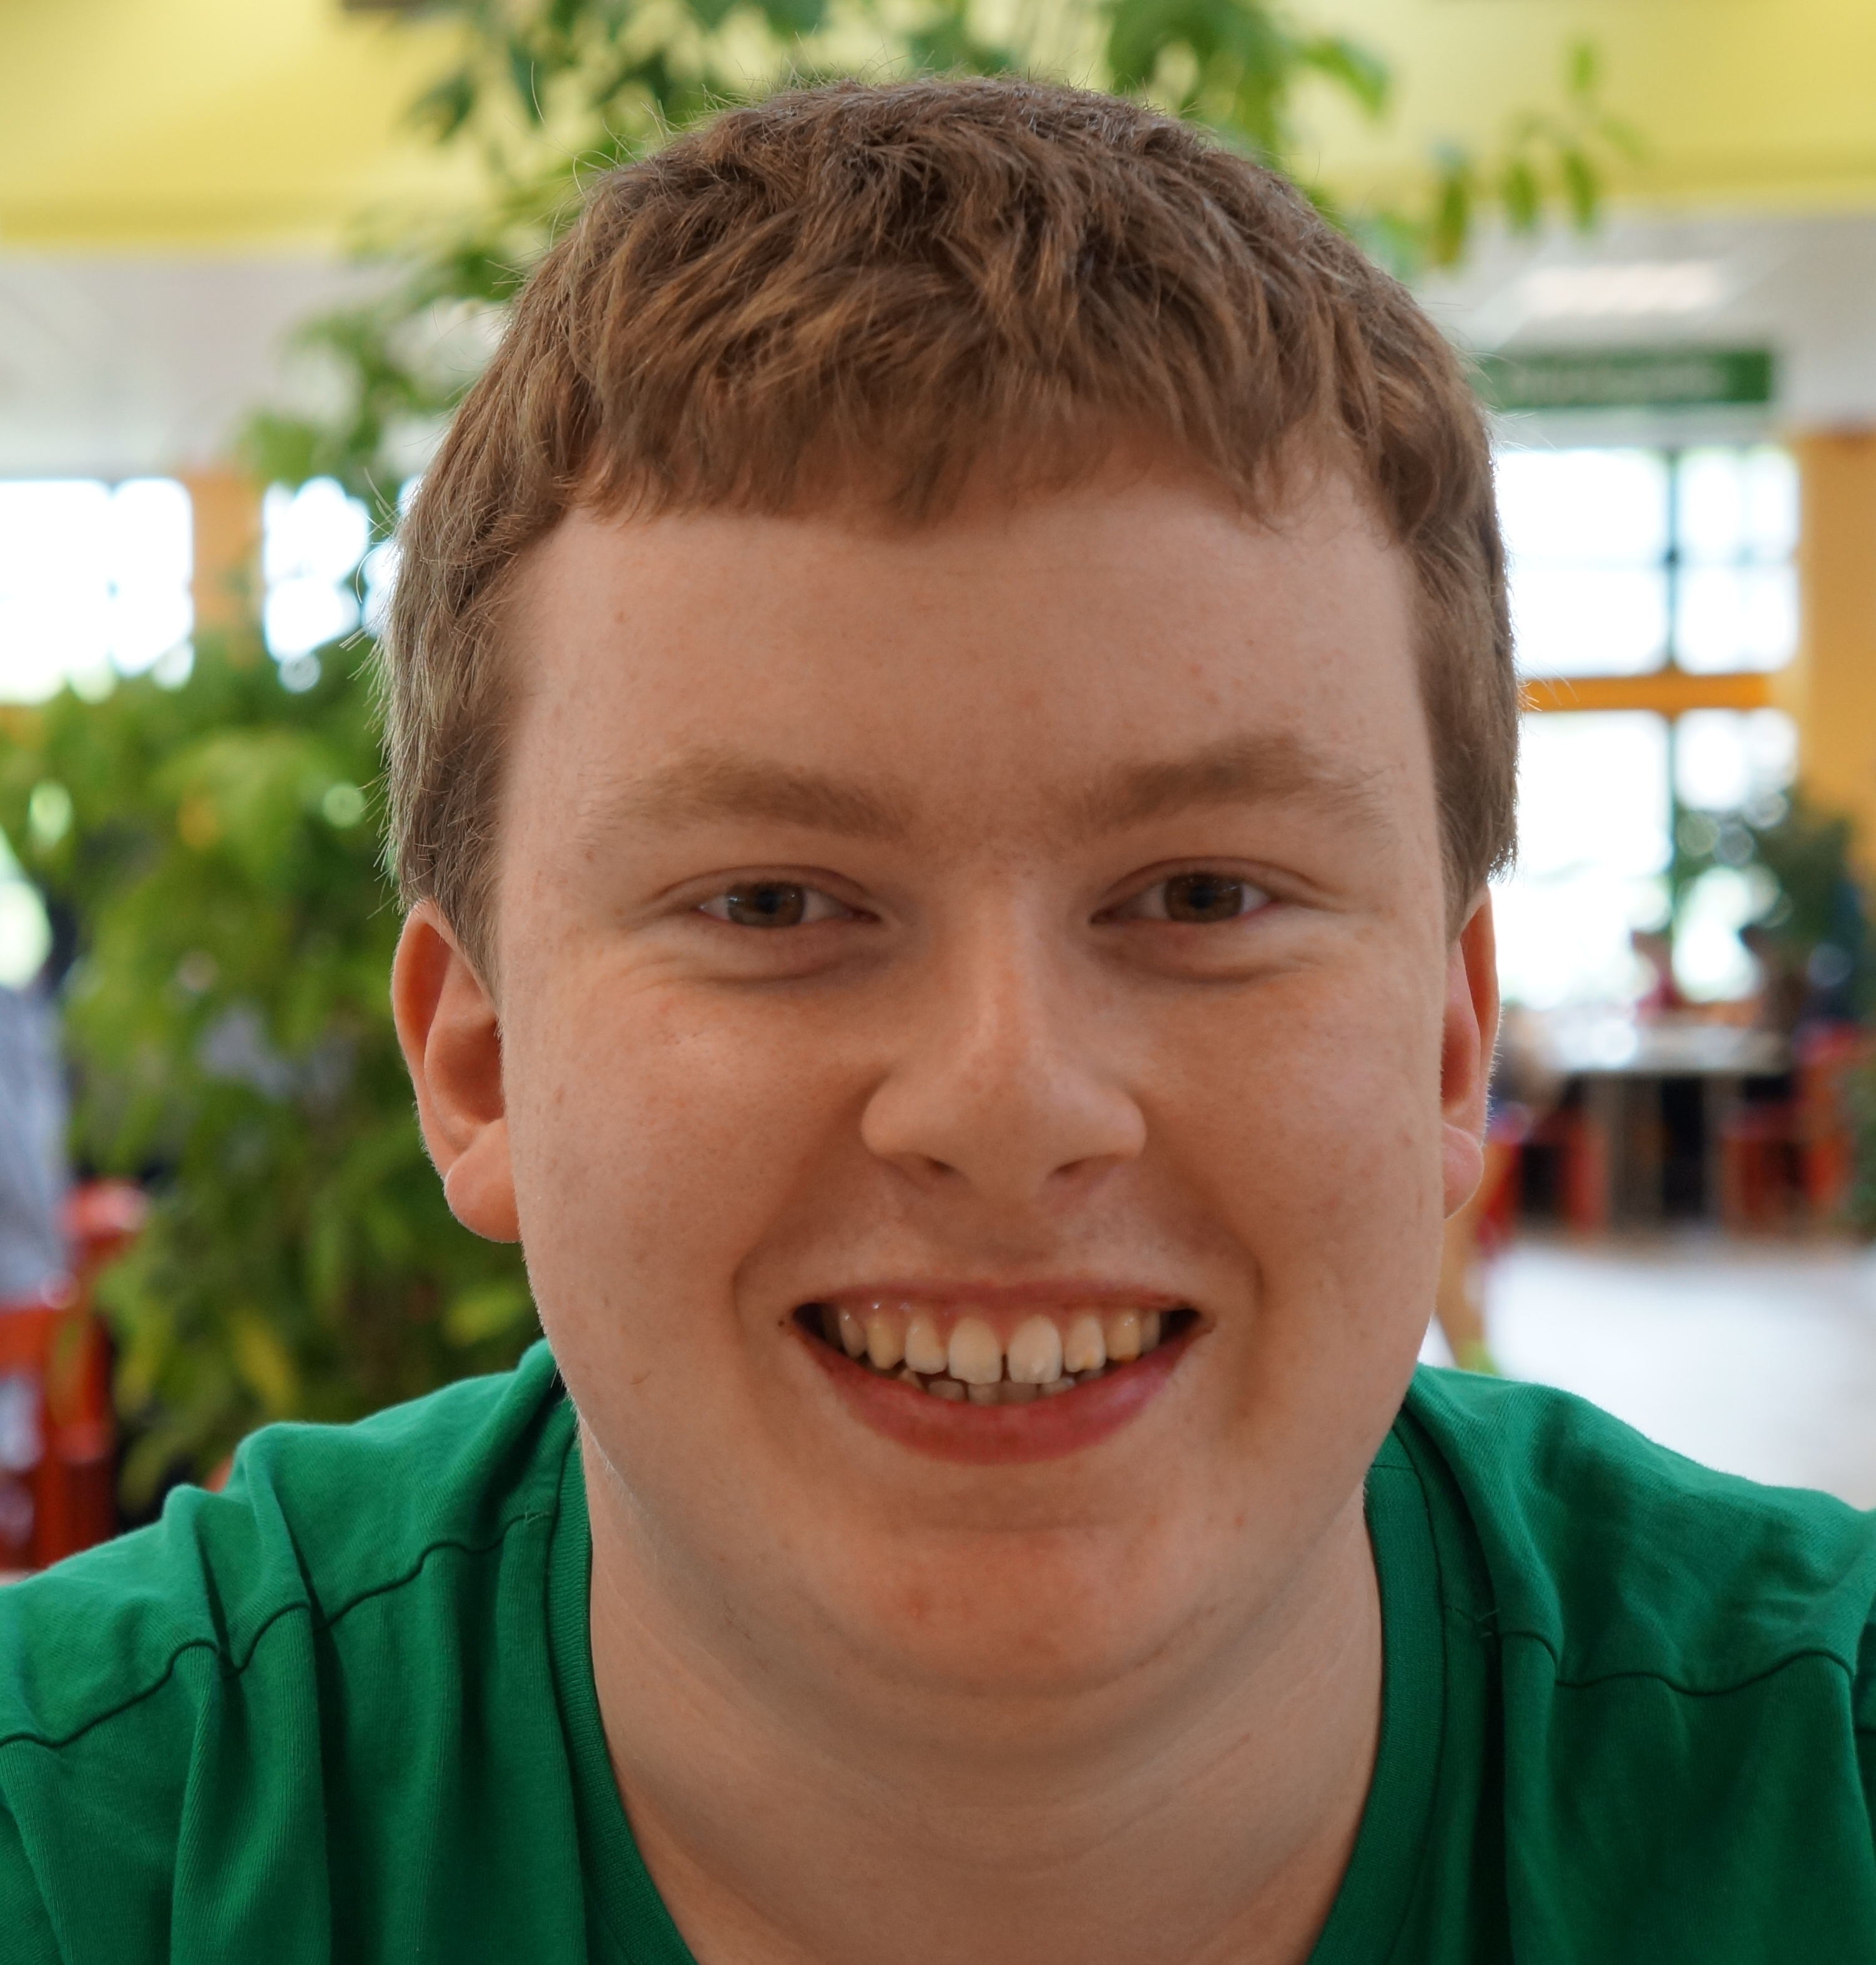
\includegraphics[width=\fibelstdlen]{res/vorstellungsfotos/maik_stappers_cropped.jpg}
	\end{wrapfigure}
}
{Heyho, ich bin Maik, arbeite seit kurzem an meiner Masterarbeit und bin seit 4~Jahren Teil dieses verrückten Haufens.
Ich befasse mich hauptsächlich mit der Interessensvertretung in Gremien, bin aber auch in die Orga der O-Woche und Ersti-Fahrt involviert.}

\fibelvorstellung{
	\begin{wrapfigure}{l}{0cm}
		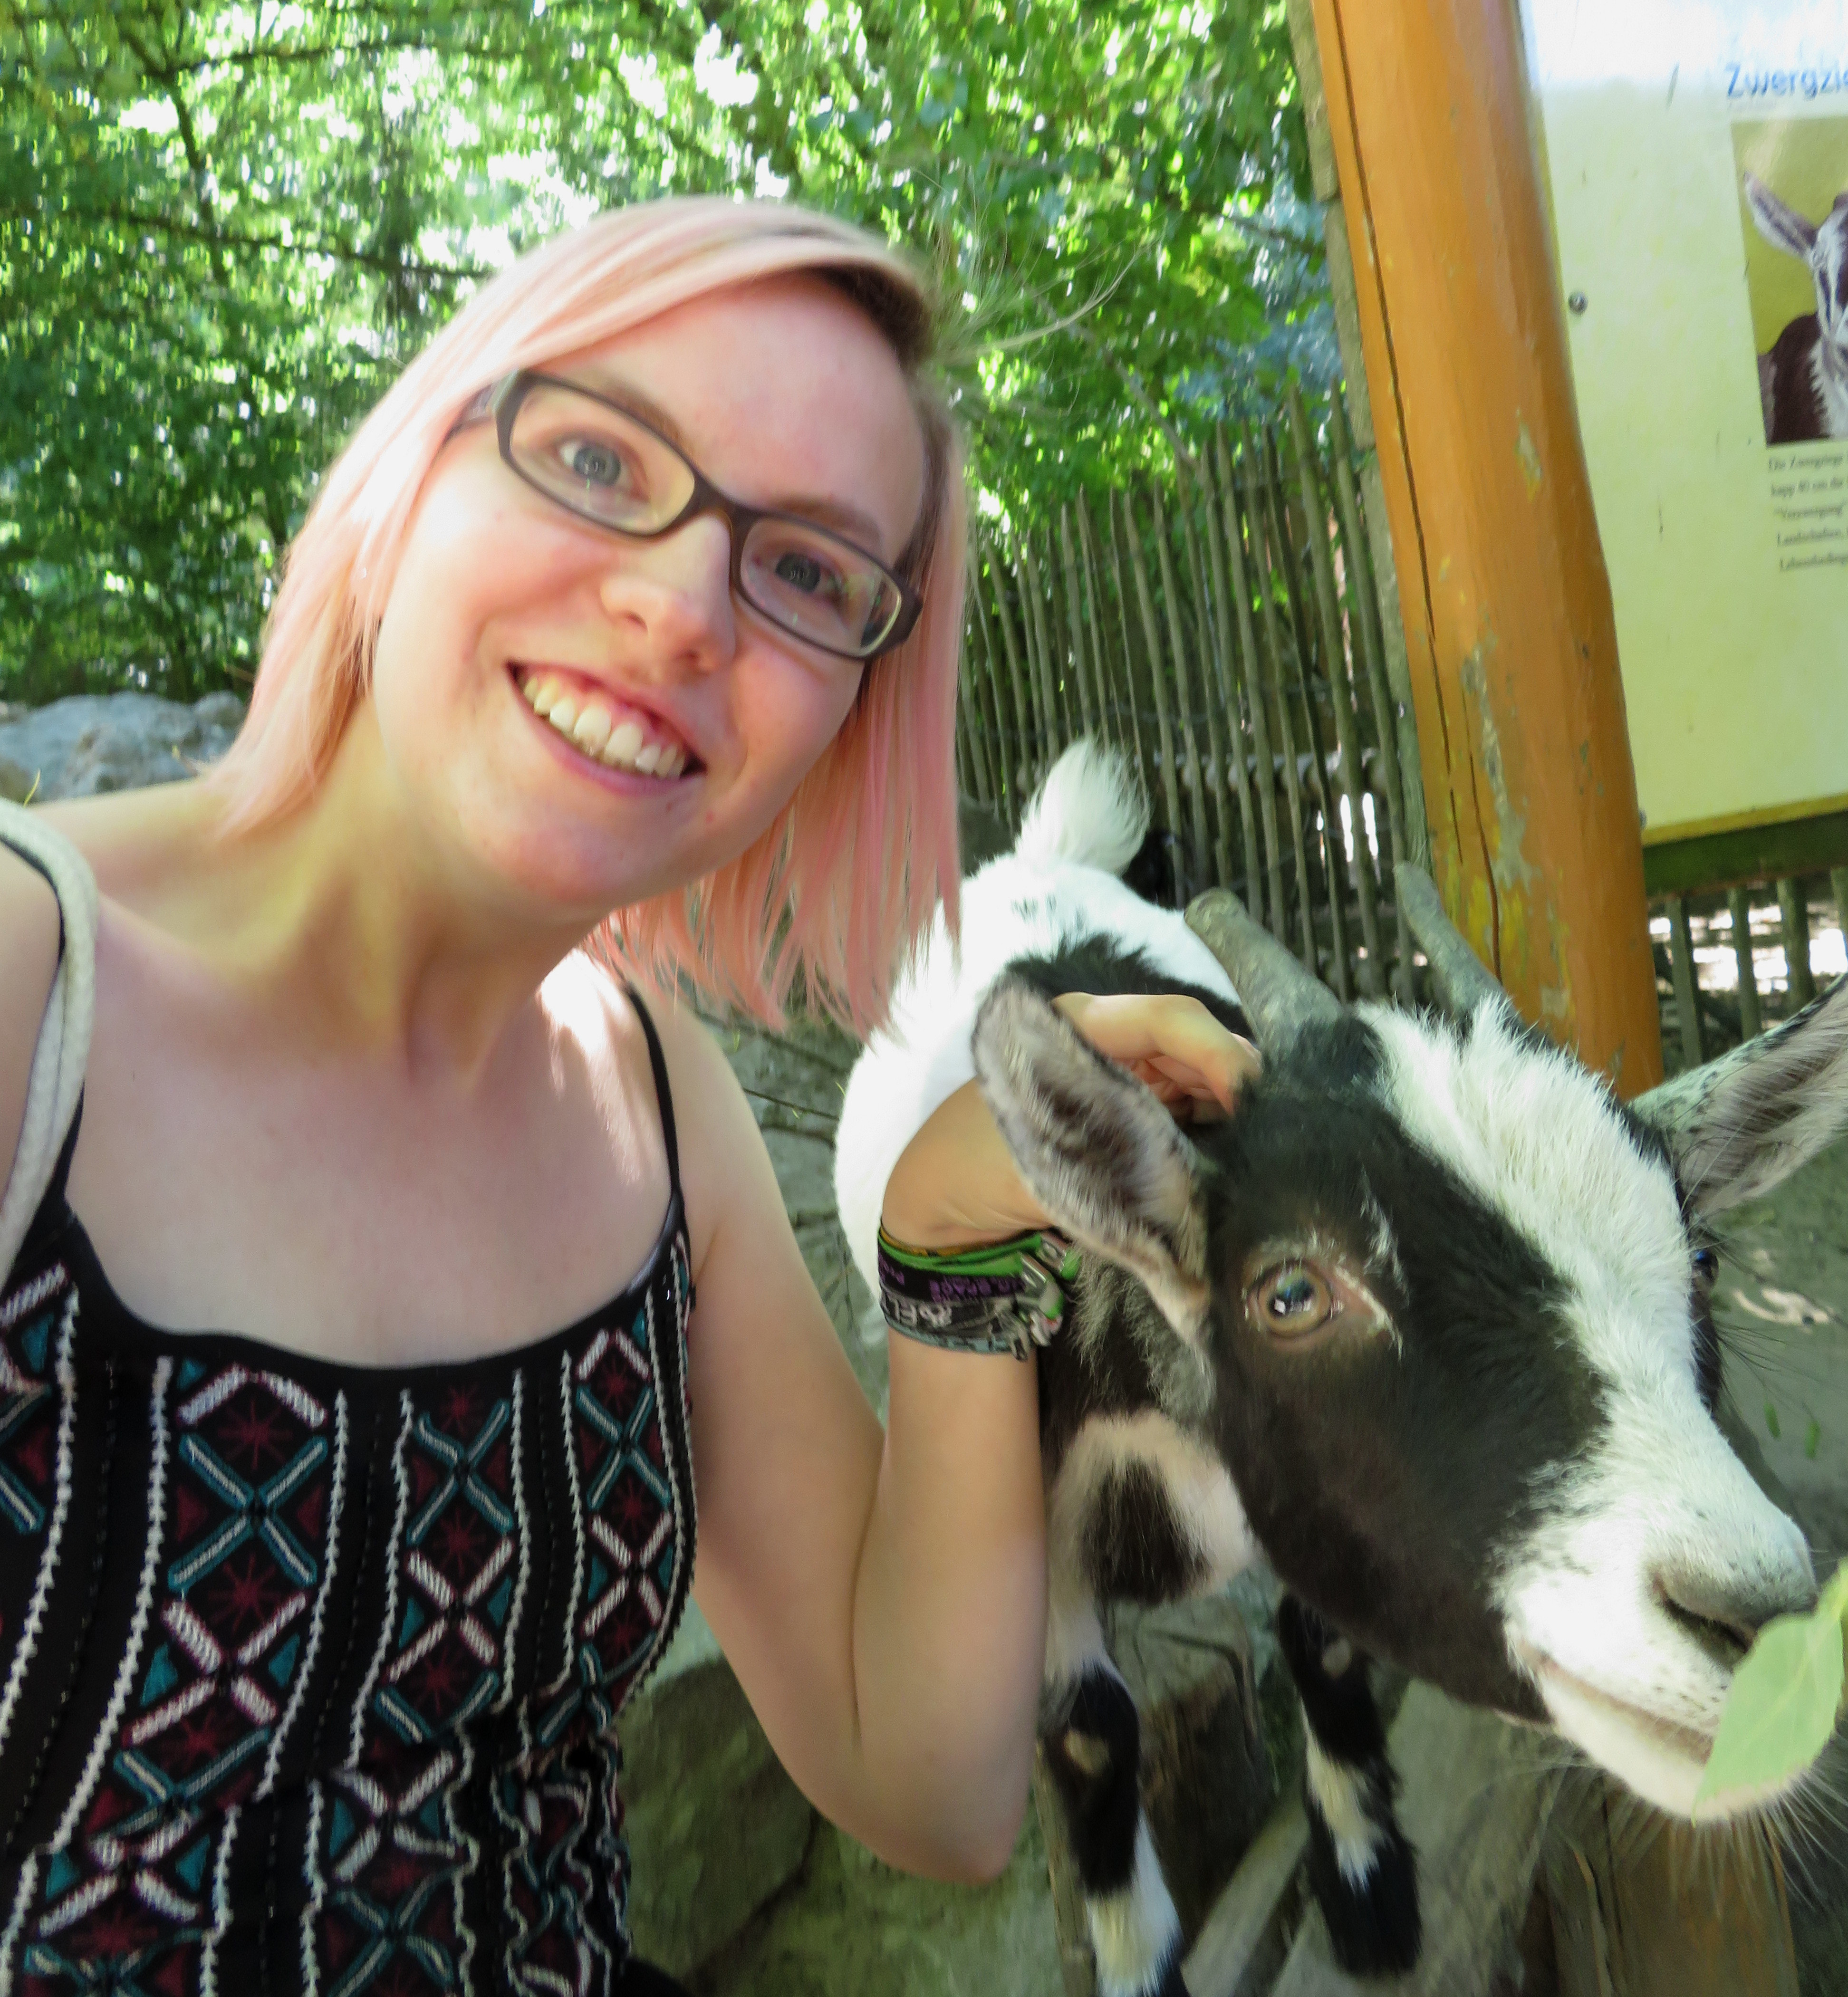
\includegraphics[width=\fibelstdlen]{res/vorstellungsfotos/miriam_neumann_cropped.jpg}
	\end{wrapfigure}
}
{Hey, ich bin Miri, im 5.~Semester und seit Anfang an in der Fachschaft aktiv.
Bei einem Tee (oder Bierchen) könnt ihr gerne mit mir über das Studium, den Beginn in einer neuen Stadt oder einfach mal so reden.
% XXX warum geht der Text am Seitenende ein bisschen über den Rand?
\vspace{1ex}}

\fibelvorstellung{
	\begin{wrapfigure}{r}{0cm}
		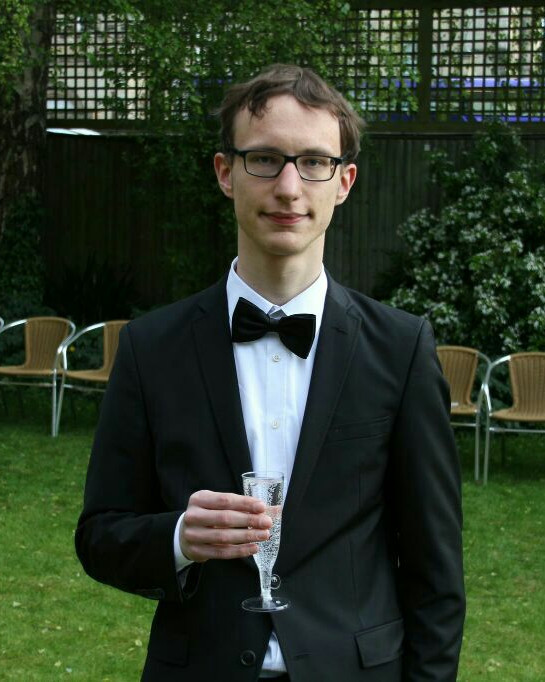
\includegraphics[width=\fibelstdlen]{res/vorstellungsfotos/michael_te_vrugt_cropped.jpg}
	\end{wrapfigure}
}
{Hi, ich bin Michael und studiere im 5.~Semester Physik und Philosophie.
Dass ihr mich bislang noch nicht getroffen habt, liegt daran, dass ich momentan ein Auslandsjahr an der Universität Oxford einlege.
Ihr könnt mir aber jederzeit eine Mail schreiben, falls ihr Fragen zu Philosophie, einem Doppelstudium oder Stipendien habt.
Ansonsten wünsche ich euch viel Spaß und Erfolg im Studium.}

\fibelvorstellung{
	\begin{wrapfigure}{l}{0cm}
		\includegraphics[width=\fibelstdlen]{res/vorstellungsfotos/philip_render_cropped.png}
	\end{wrapfigure}
}
{Hi, ich bin der Philip. Bin schon ein bisschen länger an der Uni und oft an der charakteristischen Bierpulle zu erkennen ;)

Als 2FB kann ich euch auch übrigens immer gut von den schönen Seiten des Physikstudiums berichten.
\vspace{\baselineskip}}

\fibelvorstellung{
	\begin{wrapfigure}{r}{0cm}
		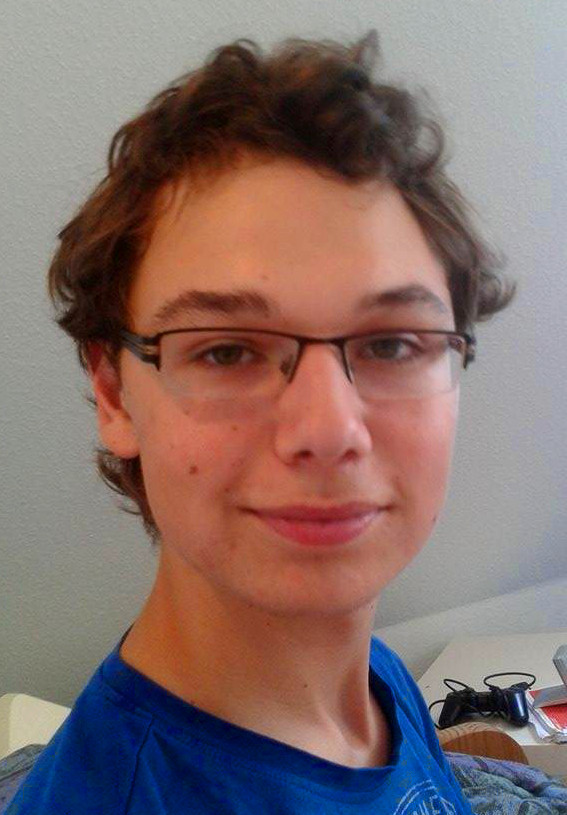
\includegraphics[width=3.2cm]{res/vorstellungsfotos/rene_henke.jpg}
	\end{wrapfigure}
}
{Ich bin der René (nicht zu verwechseln mit Rene) und studiere momentan Physik im 5.~Semester.
	Neben der Fachschaft bin ich auch in der jDPG Regionalgruppe Münster aktiv, stehe also gerne als Ansprechpartner für alles, was die jDPG betrifft, zur Seite.
	\vspace{\baselineskip}}

\fibelvorstellung{
	\begin{wrapfigure}{l}{0cm}
		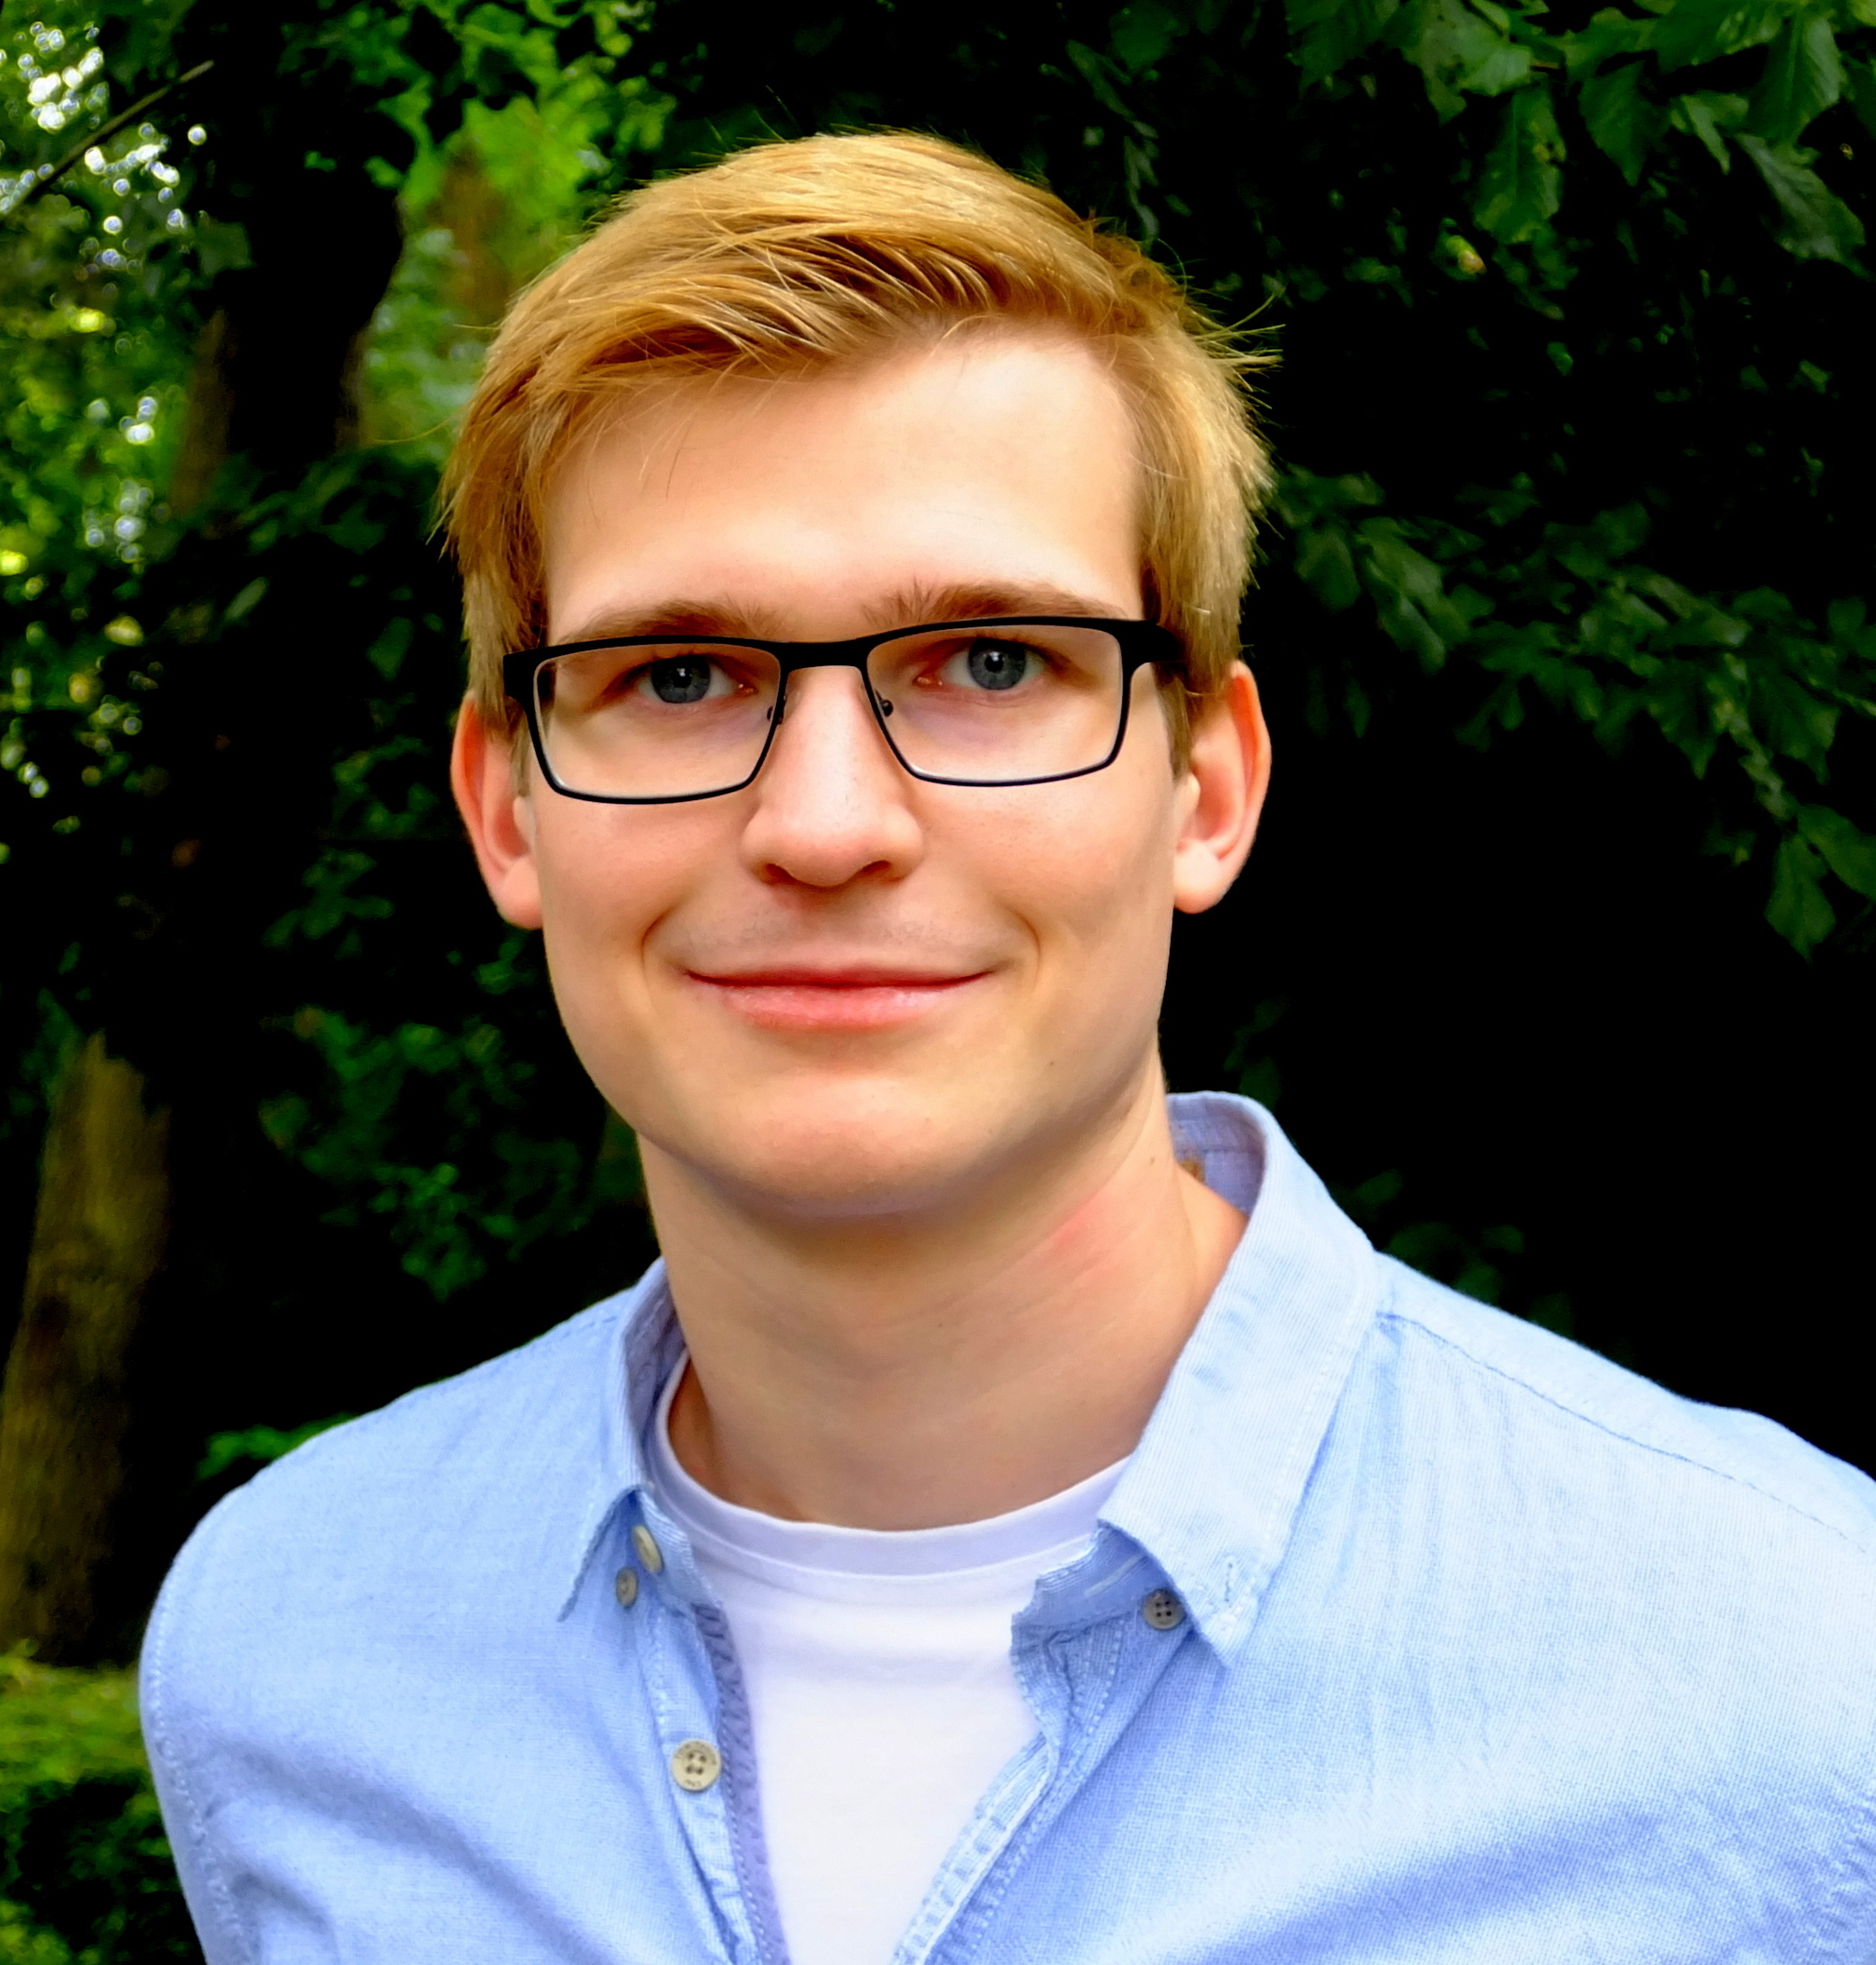
\includegraphics[width=\fibelstdlen]{res/vorstellungsfotos/rene_ross_cropped.jpg}
	\end{wrapfigure}
}
{Hi, ich bin Rene und studiere jetzt im 2.~Semester Master Physik.
Ich bin damals kurz nach der O-Woche zur Fachschaft gestoßen und seitdem durchgehend dabei und kann euch also mit Rat und Tat bei euren Fragen helfen.}

\fibelvorstellung{
	\begin{wrapfigure}{r}{0cm}
		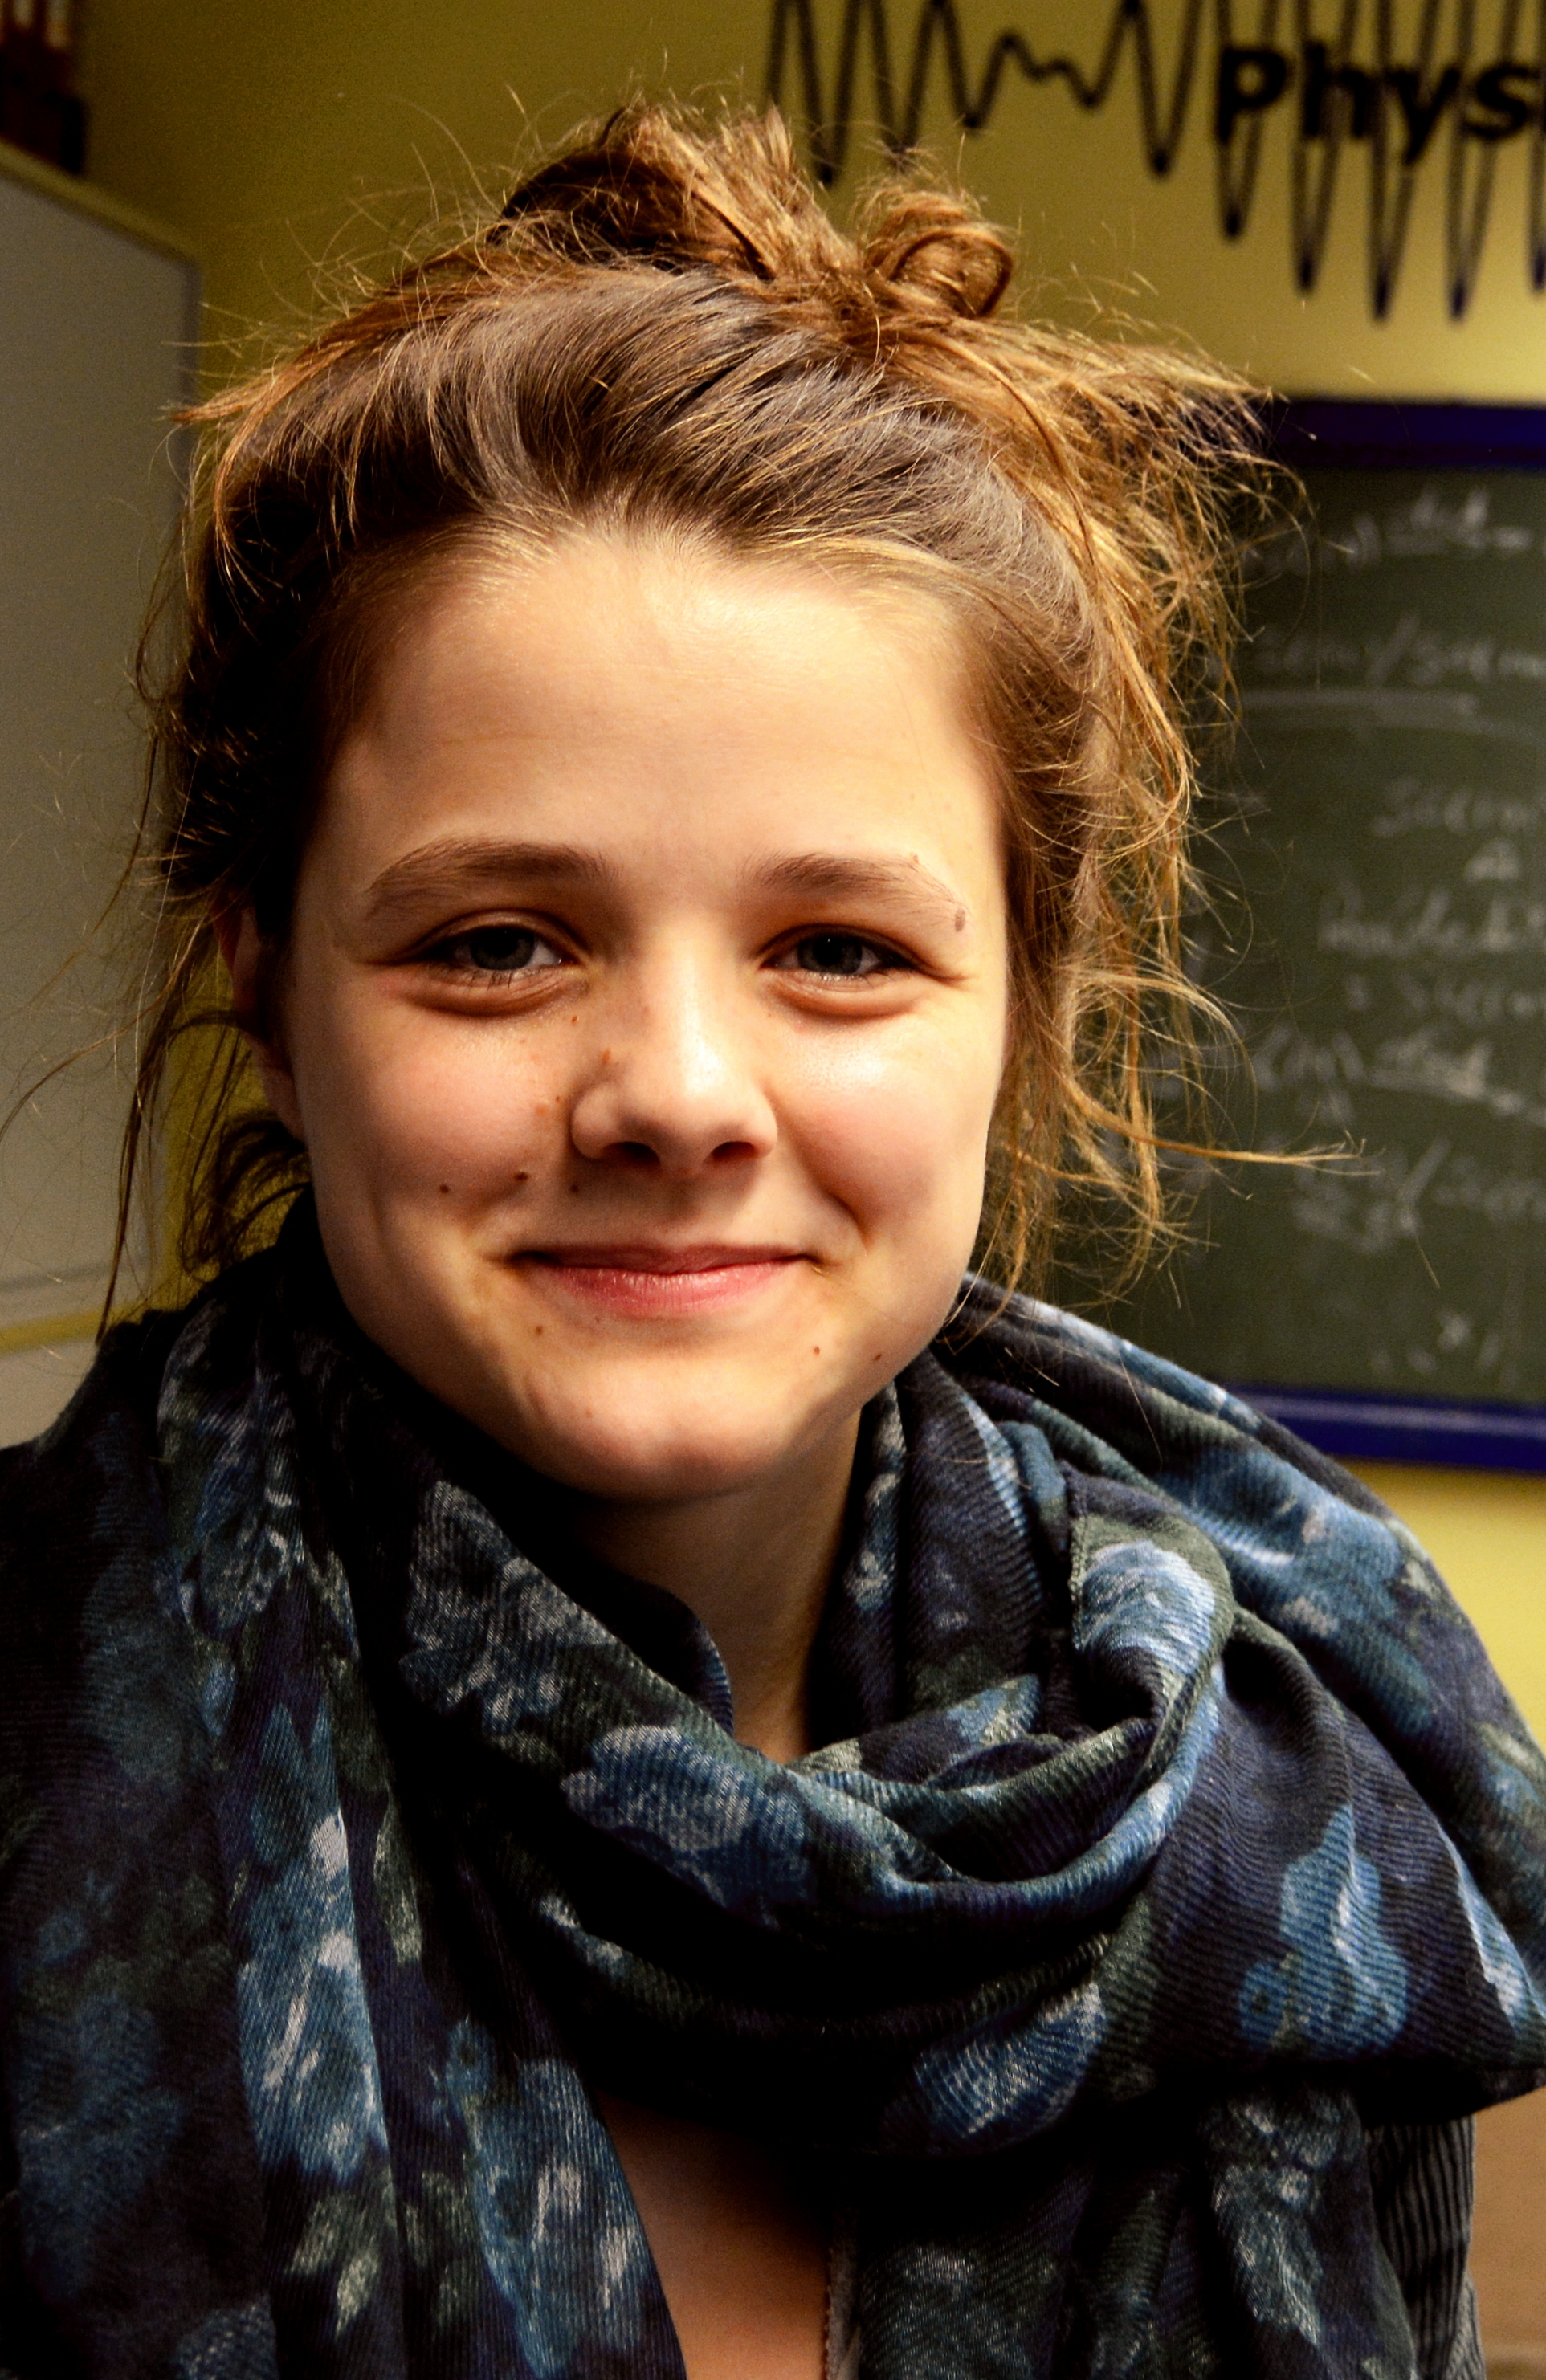
\includegraphics[width=\fibelstdlen]{res/vorstellungsfotos/pia_petrak_cropped.jpg}
	\end{wrapfigure}
}
{Hi, ich bin Pia, 19/20 (direkt in der Ersti-Woche), 1-Fach-Bachelor Physik 2./3.\ Semester. Ein Glück, dass ihr endlich da seid!
	So muss ich mir nicht länger anhören, dass ich ja immer noch Ersti sei trotz 2.~Semesters, weil ja immer nur zum Wintersemester neue Physikstudierende dazukommen.
	Im Übrigen: Physik ist wirklich cool ;)\\
	Und verpasst bloß nix von der Erstiwoche!
	Die fand ich "damals" nämlich ziemlich cool.}

\vspace{6ex}

\fibelvorstellung{
	\begin{wrapfigure}{l}{0cm}
		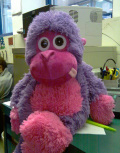
\includegraphics[width=\fibelstdlen]{res/vorstellungsfotos/fritz.png}
	\end{wrapfigure}
}
{Hallo, ich bin Fritz und bin neu in der Fachschaft Physik.
Die Mannschaft hier ist echt genial aufgestellt, sodass es richtigen Spaß macht, ein aktiver Teil der Universität Münster zu sein.
Ich kann dir nur empfehlen: Mach' mit und verändere die Uni!}

\vspace{\fill}

\includegraphics[width=\columnwidth]{private/res/nichtlustig/140505_volker.jpg}

\vspace{7ex}
\end{multicols*}
